
\documentclass[11pt]{beamer}
\usetheme{Frankfurt}
\usecolortheme{seahorse}
\usepackage{multirow}
\usepackage{pifont}
\usepackage{bm}
\usepackage{caption}
%\usepackage{subcaption}
\usepackage{url}


\setbeamertemplate{footline}[frame number]
\setbeamertemplate{itemize items}[triangle]
\setbeamertemplate{frametitle}[default][center]




%%% ========================================================
%% For the cover page
%% ========================================================
% la ligne ci-dessous est à insérer obligatoirement dans le préambule du document avant \begin{document}
\usepackage[a4paper]{./cover/meta-donnees} % for the title page

%% ========================================================
%% General packages
%% ========================================================

\usepackage{times,amsmath,amssymb,amsfonts,color,graphicx,latexsym,amsthm}
% \usepackage{xcolor}
\usepackage[table,dvipsnames]{xcolor}
\usepackage{booktabs} % for better tables

\usepackage{tikz,array}
\usetikzlibrary{arrows,automata,calc,decorations.pathmorphing, backgrounds,fit, shapes}

\usepackage{algorithm, algpseudocode}
\usepackage{setspace} % used with \begin{spacing}{..}..\end{spacing}  --> needed in book
% 
\usepackage[normalem]{ulem}

\usepackage{datetime}

\graphicspath{ {figures/} }
% \usepackage{caption}
\usepackage[font={small}]{caption}
\usepackage{subcaption}
% \usepackage[labelformat=simple]{subcaption}
% \renewcommand\thesubfigure{(\alph{subfigure})}  % subfigure with parenthesis, e.g., Figure 1.2(a)
% \renewcommand\thesubfigure{-\alph{subfigure}}   % subfigure with dash, e.g., Figure 1.2-a
\usepackage{multirow}
% \captionsetup{justification=centering}
% \usepackage[caption=true]{subfig}

\usepackage{enumitem} % to change list styling globally

%% ========================================================
% % for the geometry of the pages
%% ========================================================
% \setlength{\parindent}{3.0em}
% \setlength{\parskip}{0.5em}
% \linespread{1.1}  % space between lines
% \usepackage{fullpage}  % decrease margins
% \usepackage{a4wide}
% \usepackage{showframe}   % shows the frames of the pages

%% ========================================================
% Set depth of TOC
%% ========================================================
% \setcounter{tocdepth}{2}
% \settocdepth{subsection}
% \setsecnumdepth{subsection}

%% ========================================================
%% for the mini-toc - have a toc in the beginning of each chapter
%% ========================================================
% \usepackage{minitoc}
% \setcounter{minitocdepth}{1} 
%\nomtcrule       % removes rules = horizontal lines
%\nomtcpagenumbers  % remove page numbers from minitocs
% \dominitoc %% \dominitoc[n] removes contents, \dominitoc[c] centers contents


%% ========================================================
% % %% Make an index list
%% ========================================================
% % \usepackage{imakeidx}
% % \makeindex[title=Index, options= -s ./stylefiles/myIndexStyle.ist, intoc, columns=1]


%% ========================================================
%%%% Style of Chapters 
%% ========================================================

% \usepackage[Lenny]{fncychap}
% \usepackage[Sonny]{fncychap}
% \usepackage[Rejne]{fncychap}
% \usepackage[Bjarne]{fncychap}
% \usepackage[Bjornstrup]{fncychap}
% \usepackage[Conny]{fncychap} %%  incompatible with toc


%% My STYLE
%% Set introduction chapter to 0
% \setcounter{chapter}{-1}

%% My STYLE 
\usepackage{fancyhdr}
\addtolength{\headheight}{\baselineskip}
\fancyhead{} % clear all header fields
\fancyhead[RE]{\leftmark}
\fancyhead[LO]{\rightmark}
\fancyhead[LE,RO]{\thepage}
\fancyfoot{} % clear all footer fields
\fancyfoot[RO,LE]{\textcolor{gray}{\today\ (\currenttime)}}

\usepackage{titlesec}
% % % % % \titleformat{command}[shape]{format}{label}{sep}{before}[after]
% % % % % \titlespacing{<command>}{<left>}{<before-sep>}{<after-sep>}[<right>]

%%%%%%%%%%%%%%%%%%%%%%%%%%%%%%%%%%%%%%%%%%%%%%%%%%%%%%%%%%%%%%%%%%%
%%%%% % Simple Chapter title aligned right
% \titleformat{\chapter}[display]{\color{black}\normalfont\LARGE\bfseries\raggedleft}{\chaptertitlename\ \thechapter}{20pt}{\Huge}

%%%%%%%%%%%%%%%%%%%%%%%%%%%%%%%%%%%%%%%%%%%%%%%%%%%%%%%%%%%%%%%%%%%
%%%%% white Chapter number on black box
% \titleformat{\chapter}[display]{\color{black}\normalfont\LARGE\bfseries\raggedleft}{\textsc{\chaptertitlename}\ \marginpar{\fontsize{50}{60}\selectfont\textcolor{white}{\colorbox{black!50}{\makebox(64,64)\thechapter}}}}{20pt}{\Huge}

%%%%%%%%%%%%%%%%%%%%%%%%%%%%%%%%%%%%%%%%%%%%%%%%%%%%%%%%%%%%%%%%%%%
%%% calligraphic Chapter number in the margin (aurical)
% \usepackage{aurical}
% \usepackage[T1]{fontenc}
% \titleformat{\chapter}[display]{\color{black}\normalfont\LARGE\bfseries\raggedleft}{\textsc{\chaptertitlename}\ \marginpar{\hspace{-1em}\Fontauri\fontsize{100}{120}\selectfont\textcolor{black!30}{\thechapter}}}{20pt}{\Huge}

%%%%% calligraphic Chapter number in the margin (humanist)
% \usepackage{humanist}
% \usepackage[T1]{fontenc}
% \titleformat{\chapter}[display]{\color{black}\normalfont\LARGE\bfseries\raggedleft}{\textsc{\chaptertitlename}\ \marginpar{\hminfamily \fontsize{100}{120}\selectfont\textcolor{black!30}{\thechapter}}}{20pt}{\Huge}

% %%%%%% calligraphic Chapter number in the margin (square caps)
% \usepackage{sqrcaps}
% \usepackage[T1]{fontenc}
% \titleformat{\chapter}[display]{\color{black}\normalfont\LARGE\bfseries\raggedleft}{\textsc{\chaptertitlename}\ \marginpar{\sqrcfamily \fontsize{75}{90}\selectfont\textcolor{black!40}{\colorbox{black!10}{\mbox{\thechapter}}}}}{20pt}{\Huge}

%%%%%%%%%%%%%%%%%%%%%%%%%%%%%%%%%%%%%%%%%%%%%%%%%%%%%%%%%%%%%%%%%%%
%%%%% %%% Big Gray Chapter number in the margin
% \titleformat{\chapter}[display]{\color{black}\normalfont\LARGE\bfseries\raggedleft}{\textsc{\chaptertitlename}\ \marginpar{\fontsize{100}{120}\selectfont\textcolor{black!30}{\thechapter}}}{20pt}{\Huge}

%%%%%%%%%%%%%%%%%%%%%%%%%%%%%%%%%%%%%%%%%%%%%%%%%%%%%%%%%%%%%%%%%%%
%%%%% %% white Chapter number on gray box in the margin - with vertical ``chapter''
% \titleformat{\chapter}[display]{\color{black}\normalfont\LARGE\bfseries\raggedleft}{\rotatebox{90}{\textsc{\chaptertitlename}}\ \marginpar{\hspace{-.7em}\fontsize{60}{72}\selectfont\textcolor{white}{\colorbox{black!50}{\makebox(64,80)\thechapter}}}}{.5em}{\Huge}

% %% white Chapter number on gray box - with vertical ``chapter''
% \titleformat{\chapter}[display]{\color{black}\normalfont\LARGE\bfseries\raggedleft}{\rotatebox{90}{\textsc{\chaptertitlename}}\ {\fontsize{60}{72}\selectfont\textcolor{white}{\colorbox{black!50}{\makebox(64,80)\thechapter}}}}{.5em}{\Huge}

% %% white Chapter number on black box inline- with vertical ``chapter''
\titleformat{\chapter}[display]{\color{black}\normalfont\LARGE\bfseries\raggedleft}{\rotatebox{90}{\textsc{\chaptertitlename}}\ {\hspace{0em}\fontsize{60}{72}\selectfont\textcolor{black!80}{\colorbox{red!20!black!10}{\makebox(64,80)\thechapter}}}}{.5em}{\Huge}


%% ========================================================
%%% Add background to all figures
%% ========================================================
% 
% \usepackage{mdframed}
% 
% \let\originalfigure=\figure
% \let\endoriginalfigure=\endfigure
% 
% \renewenvironment{figure}[1][]{
%   \begin{originalfigure}[#1]
%     \begin{mdframed}[linecolor=black!5,backgroundcolor=black!5]
% }{
%     \end{mdframed}
%   \end{originalfigure}
% }

%% ========================================================
%% Hyperef
%% ========================================================

\usepackage[pagebackref=true]{hyperref} % load hyperref last 
\hypersetup{linktocpage,linktoc=all}
\hypersetup{colorlinks=true,linkcolor=blue,urlcolor=blue,citecolor=blue,filecolor=blue}

% for adding backreference in the bibliography
\renewcommand*{\backref}[1]{}
\renewcommand*{\backrefalt}[4]{({\it%
    \ifcase #1 Not cited.%
          \or Cited on page~#2.%
          \else Cited on pages #2.%
    \fi%
    })}
% Symbols
\newcommand{\ra}{\rightarrow}
\newcommand{\ov}{\overline}
\newcommand{\ur}{\underline}
\newcommand{\pr}{\prime}
\newcommand{\tbf}{\textbf}
\newcommand{\omg}{\Omega}
\newcommand{\mc}{\mathcal}
\newcommand{\lt}{\left}
\newcommand{\rt}{\right}
\newcommand{\mb}{\mathbb}
\newcommand{\imp}{\implies}
\newcommand{\dimp}{\Leftrightarrow}
\newcommand{\wh}{\widehat}
\newcommand{\dg}{\mc{D}}


% Sets
\newcommand{\realset}{\mb{R}}
\newcommand{\comprealset}{\mb{\ov{R}}}
\newcommand{\pint}{\mb{Z}_{> 0}}
\newcommand{\nzrl}{\mb{R}_{\geq 0}}
\newcommand{\prl}{\mb{R}_{>0}}
\newcommand{\rl}{\mb{R}}
\newcommand{\fin}{\forall i\in\{1,...,n\}}
\newcommand{\tup}[1]{\{1,...,#1\}}
\newcommand{\seq}[2]{_{#1=1}^#2}
\newcommand{\mCnn}{\mb{M}_{n\times n}(\mb{C})}
\newcommand{\mCmm}{\mb{M}_{m\times m}(\mb{C})}
\newcommand{\mCpn}{\mb{M}_{p\times n}(\mb{C})}
\newcommand{\mCnm}{\mb{M}_{n\times m}(\mb{C})}
\newcommand{\mRnn}{\mb{M}_{n\times n}(\mb{R})}
\newcommand{\mRpn}{\mb{M}_{p\times n}(\mb{R})}
\newcommand{\mRnm}{\mb{M}_{n\times m}(\mb{R})}
\newcommand{\mRno}{{{\mb{R}}}^n_{\geq 0}}
\newcommand{\mRmo}{{{\mb{R}}}^m_{\geq 0}}
\newcommand{\mRo}{\mb{R}_{\geq 0}}
\newcommand{\mRn}{{\mb{R}}^n}
\newcommand{\mRm}{{\mb{R}}^m}
\newcommand{\mCn}{\mb{C}^n}
\newcommand{\mCm}{\mb{C}^m}
\newcommand{\inv}{\mb{GL}_n(\mb{R})}
\newcommand{\id}[1]{\mb{I}_{#1\times #1}}
\newcommand{\mat}[3]{\mb{M}_{#1\times #2}(\mb{#3})}


% matrix operations
\newcommand{\ColumnJoin}[2]{\left[\begin{array}{l}{#1}\\{#2} \end{array}\right]}
\newcommand{\minaffine}[2]{\Lambda^{\min}\lt(#1,#2\rt)}
\newcommand{\maxaffine}[2]{\Lambda^{\max}\lt(#1,#2\rt)}

% local macros
\DeclareMathOperator{\real}{\operatorname{Re}}
\newcommand{\CZ}{\lt(V,c,s\rt)}
\newcommand{\GCZ}{\gcz{V}{c}{s}{W}{l}{u}}
\newcommand{\cz}[3]{\mc{C}\lt(#1,#2,#3\rt)}
\newcommand{\CZO}{\lt(V,0,s\rt)}
\newcommand{\czo}[2]{\mc{Z}\lt(#1,0,#2\rt)}
\newcommand{\trj}[2]{{\bf #1}(#2)}
\newcommand{\IncTcz}[6]{\mc{T}\lt(#1,#2,#3,#4,#5,#6\rt)}
\newcommand{\IncGcz}[6]{\mc{G}\lt(#1,#2,#3,#4,#5,#6\rt)}
\newcommand{\Ptope}[3]{\mc{P}\left(#1,#2,#3\right)}
\newcommand{\gcz}[6]{\mathcal{Z}\lt(#1,#2,#3,#4,#5,#6\rt)}
\newcommand{\sptope}[3]{\mathcal{P}\lt(#1,#2,#3\rt)}
\newcommand{\system}{\mb{H}}
\newcommand{\locationset}{Q}
\newcommand{\edgeset}{E}
\newcommand{\stay}{\gamma}
\newcommand{\linearmapset}{\mc{A}}
\newcommand{\inputset}{U}
\newcommand{\initialset}{\Omega}
\newcommand{\edge}{\sigma}
\newcommand{\loc}{q}
\newcommand{\map}{\linearmapset}
\newcommand{\inp}{\inputset}
\newcommand{\ptemplate}{\mc{K}}
\newcommand{\systrj}[2]{\lt({\bf #1},{\bf #2}\rt)}
\newcommand{\wholenums}{\mb{Z}_\geq 0}
\newcommand{\preloc}[1]{#1_{1}}
\newcommand{\postloc}[1]{#1_{2}}
\newcommand{\upperedgebound}[1]{#1^+}
\newcommand{\loweredgebound}[1]{#1^-}
\newcommand{\reset}[1]{#1_r}
\newcommand{\locationtransition}[1]{R_{#1}}
\newcommand{\edgetransition}[1]{R_{#1}}
\newcommand{\staysptope}[1]{\sptope{\ptemplate\lt(#1\rt)}{\stay^-\lt(#1\rt)}{\stay^+\lt(#1\rt)}}
\newcommand{\guardsptope}[1]{\sptope{\ptemplate\lt(\preloc{#1}\rt)}{\max\lt(\loweredgebound{#1},\stay^-\lt(\preloc{#1}\rt)\rt)}{\min\lt(\upperedgebound{#1},\stay^+\lt(\preloc{#1}\rt) \rt)}}
\newcommand{\hybridset}{\Gamma}
\newcommand{\transfer}[4]{#1#4 = #2\dg\lt(#3\rt)}
\newcommand{\centertransfer}[4]{#1#4 = #3-#2}
\newcommand{\scalebound}[5]{\max_{i=1}^{#4}\lt(\lt(\sum_{j=1}^{#5}\lt|#1\rt|_j\rt)-#3_i+#2_i\rt)}
\newcommand{\pseudoinverse}[1]{#1\lt(#1#1^T\rt)^{-1}}

\newcommand{\mb}{\mathbb}
\newcommand{\mCnn}{\mb{M}_{n\times n}(\mb{C})}
\newcommand{\mCmm}{\mb{M}_{m\times m}(\mb{C})}
\newcommand{\mCpn}{\mb{M}_{p\times n}(\mb{C})}
\newcommand{\mCnm}{\mb{M}_{n\times m}(\mb{C})}
\newcommand{\mRnn}{\mb{M}_{n\times n}(\mb{R})}
\newcommand{\mRpn}{\mb{M}_{p\times n}(\mb{R})}
\newcommand{\mRnm}{\mb{M}_{n\times m}(\mb{R})}
\newcommand{\mRno}{{{\mb{R}}}^n_{\geq 0}}
\newcommand{\omRno}{{\ov{\mb{R}}}^n_{\geq 0}}
\newcommand{\mRmo}{{{\mb{R}}}^m_{\geq 0}}
\newcommand{\omRmo}{{\ov{\mb{R}}}^m_{\geq 0}}
\newcommand{\mRo}{\mb{R}_{\geq 0}}
\newcommand{\omRo}{\ov{\mb{R}}_{\geq 0}}
\newcommand{\mRn}{{\mb{R}}^n}
\newcommand{\omRp}{{\ov{\mb{R}}}^p}
\newcommand{\mRm}{{\mb{R}}^m}
\newcommand{\omRm}{\ov{\mb{R}}^m}
\newcommand{\mCn}{\mb{C}^n}
\newcommand{\mCm}{\mb{C}^m}


\definecolor{magenta(dye)}{rgb}{0.79, 0.08, 0.48}
\definecolor{calpolypomonagreen}{rgb}{0.12, 0.3, 0.17}
\definecolor{coolblack}{rgb}{0.0, 0.18, 0.39}
\definecolor{palatinatepurple}{rgb}{0.41, 0.16, 0.38}
\definecolor{pansypurple}{rgb}{0.47, 0.09, 0.29}
\definecolor{prune}{rgb}{0.44, 0.11, 0.11}
\definecolor{outrageousorange}{rgb}{1.0, 0.43, 0.29}
\definecolor{mediumjunglegreen}{rgb}{0.11, 0.21, 0.18}
\definecolor{lincolngreen}{rgb}{0.11, 0.35, 0.02}
\definecolor{forestgreen(traditional)}{rgb}{0.0, 0.27, 0.13}
\definecolor{darksienna}{rgb}{0.24, 0.08, 0.08}
\definecolor{carminepink}{rgb}{0.92, 0.3, 0.26}
\definecolor{byzantium}{rgb}{0.44, 0.16, 0.39}
\definecolor{aureolin}{rgb}{0.99, 0.93, 0.0}
\definecolor{carrotorange}{rgb}{0.93, 0.57, 0.13}
\definecolor{daffodil}{rgb}{1.0, 1.0, 0.19}
\definecolor{darklava}{rgb}{0.28, 0.24, 0.2}
\definecolor{caputmortuum}{rgb}{0.35, 0.15, 0.13}
\definecolor{bulgarianrose}{rgb}{0.28, 0.02, 0.03}
\definecolor{armygreen}{rgb}{0.29, 0.33, 0.13}
\definecolor{darkmidnightblue}{rgb}{0.0, 0.2, 0.4}
\definecolor{darkjunglegreen}{rgb}{0.1, 0.14, 0.13}
\definecolor{darkgreen}{rgb}{0.0, 0.2, 0.13}
\definecolor{darkscarlet}{rgb}{0.34, 0.01, 0.1}
\definecolor{darkslategray}{rgb}{0.18, 0.31, 0.31}
\definecolor{darkorchid}{rgb}{0.6, 0.2, 0.8}
\definecolor{darkmidnightblue}{rgb}{0.0, 0.2, 0.4}
\definecolor{darkblue}{rgb}{0.0, 0.0, 0.55}
\definecolor{sealbrown}{rgb}{0.2, 0.08, 0.08}
\definecolor{onyx}{rgb}{0.06, 0.06, 0.06}
\definecolor{neonfuchsia}{rgb}{1.0, 0.25, 0.39}
\definecolor{indianred}{rgb}{0.8, 0.36, 0.36}
\definecolor{darkred}{rgb}{0.55, 0.0, 0.0}
\definecolor{carmine}{rgb}{0.59, 0.0, 0.09}
\definecolor{cosmiclatte}{rgb}{1.0, 0.97, 0.91}
\definecolor{snow}{rgb}{1.0, 0.98, 0.98}
\definecolor{aoe}{rgb}{0.0, 0.5, 0.0}
\definecolor{alizarin}{rgb}{0.82, 0.1, 0.26}
\definecolor{britishracinggreen}{rgb}{0.0, 0.26, 0.15}
\definecolor{armygreen}{rgb}{0.29, 0.33, 0.13}
\definecolor{dartmouthgreen}{rgb}{0.05, 0.5, 0.06}
\definecolor{deepjunglegreen}{rgb}{0.0, 0.29, 0.29}
\definecolor{forestgreen(web)}{rgb}{0.13, 0.55, 0.13}
\definecolor{forestgreen(traditional)}{rgb}{0.0, 0.27, 0.13}
\definecolor{green(html/cssgreen)}{rgb}{0.0, 0.5, 0.0}
\definecolor{darkslateblue}{rgb}{0.28, 0.24, 0.55}
\definecolor{cobalt}{rgb}{0.0, 0.28, 0.67}
\definecolor{ceruleanblue}{rgb}{0.16, 0.32, 0.75}



\makeatletter
\newcommand\titlegraphicii[1]{\def\inserttitlegraphicii{#1}}
\titlegraphicii{}
\setbeamertemplate{title page}
{
  \vbox{}
   {\usebeamercolor[fg]{titlegraphic}\inserttitlegraphic\hfill\inserttitlegraphicii\par}
  \begin{centering}
    \begin{beamercolorbox}[sep=8pt,center]{institute}
      \usebeamerfont{institute}\insertinstitute
    \end{beamercolorbox}
    \begin{beamercolorbox}[sep=8pt,center]{title}
      \usebeamerfont{title}\inserttitle\par%
      \ifx\insertsubtitle\@empty%
      \else%
        \vskip0.25em%
        {\usebeamerfont{subtitle}\usebeamercolor[fg]{subtitle}\insertsubtitle\par}%
      \fi%     
    \end{beamercolorbox}%
    \vskip1em\par
    \begin{beamercolorbox}[sep=8pt,center]{date}
      \usebeamerfont{date}\insertdate
    \end{beamercolorbox}%\vskip0.5em
    \begin{beamercolorbox}[sep=8pt,center]{author}
      \usebeamerfont{author}\insertauthor
    \end{beamercolorbox}
  \end{centering}
  %\vfill
}
\makeatother
\author{Presented by Author}
\title{Presentation Title}
\subtitle{Presentation Subtile}
\institute{Department \\ University}
\date{\today}
\titlegraphic{\includegraphics[height=1cm,width=2cm]{logo1}}
\titlegraphicii{\includegraphics[height=1cm,width=2cm]{logo2}}

\begin{document}

\begin{frame}[plain]
\maketitle
\small
{\centering\itshape Jury Members\par}
President: president\par\medskip
\begin{tabular}[t]{@{}l@{\hspace{3pt}}p{.32\textwidth}@{}}
Examiners: & examiner 1 \\
& examiner 2 \\
& examiner 3 \\
& examiner 4
\end{tabular}%
\footnotesize
\begin{tabular}[t]{@{}l@{\hspace{3pt}}p{.3\textwidth}@{}}
Supervisor 1: & supervisor \\
Supervisor 2: & supervisor
\end{tabular}%

%\setbeamercolor{title}{bg=snow}
%\setbeamercolor{title}{fg=darkblue}
\title{A Calculus of Complex Zonotopes for \\ Invariant and Stability Verification \\of Hybrid Systems}
\setbeamercolor{author}{fg=darkblue}
\author[shortname]{ {\Large  Arvind\ Adimoolam}\vspace{-2em}}
%\setbeamercolor{institute}{fg=calpolypomonagreen}
%% \institute{
%% \center
%% 
\includegraphics[scale=0.15]{figures/LogoVERIMAG.png}
%% VERIMAG 
\includegraphics[scale=0.03]{logo-uga-vo-cmjn.jpg}
%% }


\date{}

\begin{document}
\nohyphens

% Title page
\begin{frame}[plain]
\maketitle
%
%
\begin{minipage}{1\textwidth}
\vspace{-4em}
\begin{minipage}{0.3\textwidth}
\eqnemph{{\small {\it Reviewers}}}\\
\plemph{{Sylvie Putot\\
Mahesh Viswanathan}}
\end{minipage}
%
\hspace{2em}
\begin{minipage}{0.3\textwidth}
\eqnemph{{\small {\it Supervised by}}}\\
\plemph{{Thao Dang}}
\end{minipage}
%
\begin{minipage}{0.25\textwidth}
\eqnemph{{\small {\it Examiners}}}\\
\plemph{{Laurent Fribourg\\
Luc Jaulin}}
\end{minipage}
%
\end{minipage}
%
\begin{minipage}{1\textwidth}
\vspace{0.5em}
\center
%
\begin{minipage}{0.2\textwidth}

\includegraphics[scale=0.15]{figures/LogoVERIMAG.png}
\end{minipage}
%
\begin{minipage}{0.5\textwidth}
{\color{darkgreen}{\center {\large VERIMAG}\\\footnotesize \hspace{0em} University Grenoble Alpes, France\\
}}
\end{minipage}
%
\begin{minipage}{0.2\textwidth}
~~
\includegraphics[scale=0.03]{logo-uga-vo-cmjn.jpg}
\end{minipage}
%
\end{minipage}
%
\end{frame}

%=============================================================================================================================

\begin{frame}{Plan}
%
\begin{enumerate}
\begin{block}{}
\item  \plemph{Dynamics} of \plemph{embedded/cyber-physical} systems %\vspace{-1em}
%
\begin{itemize}
\item \plemph{hybrid system} models
\item \plemph{trajectory set} computation for \plemph{verification/controller synthesis}
\end{itemize}
\end{block}
%
%\emph{}
%
\item \plemph{Usual zonotope} $\rightarrow$ \plemph{Complex zonotope}
%
%% \begin{itemize}
%% \item Capture \plemph{contraction} along \plemph{complex eigenvectors}
%% \end{itemize}
%
%\emph{}
%
\item \plemph{Complex Zonotope} $\rightarrow$ \plemph{Template complex zonotope}
%% \begin{itemize}
%% \item Motivation: \plemph{better approximation} of reachable sets
%% \item Basic \posemph{operations}: linear transformation, Minkowski sum, support function
%% \item \plemph{Checking inclusion} : \posemph{convex program}
%% \end{itemize}
%
%\emph{}
%
\item \plemph{Template Complex Zonotope} $\rightarrow$ \plemph{Augmented complex zonotope}
%
%% \begin{itemize}
%% \item \posemph{Intersection} with \posemph{linear constraints}
%% \end{itemize}
%
%\emph{}
%
\begin{alertblock}
\item \plemph{Applications}:
%
\begin{itemize}
\item \plemph{Stability verification} of \plemph{networked control} systems
%\item \posemph{Computing positive invariants} of discrete time affine hybrid systems
\item \plemph{Verification of linear invariance property} of affine hybrid systems
\end{itemize}
\end{alertblock}
%
\end{enumerate}
%
\end{frame}

%==================================================================================================================================

\section{Reachable set computation}

%==================================================================================================================================

\begin{frame}{Hybrid Dynamics of Real World Systems}

\begin{minipage}{0.5\textwidth}
%% Signal with hybrid behavior:
%
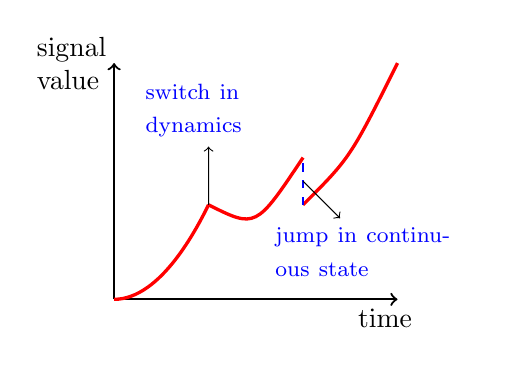
\begin{tikzpicture}[scale = 0.6]
% Create axis
\draw[thick,->] (0,0) -- (0,5);
\draw[thick,->] (0,0) -- (6,0);

% Label axis
\node[text width = 1 cm] at (-0.8,5) {signal value};
\node[text width = 1 cm] at (6,-0.4) {time};

% Create curve 1 from t=0 to t=2
\draw[red,very thick] (0,0) parabola (2,2);
% Create curve 1 from t=2 to t=4
\draw[red,very thick] (2,2) .. controls (3,1.5) .. (4,3);
% Create curve 1 from t=4 to t=6
\draw[red,very thick] (4,2) .. controls (5,3) .. (6,5);

% Label behavior of curves

% Label switch in dynamics
\node[text width = 1.6cm, blue] at (2,4)  (switch) {{\footnotesize switch in\\ dynamics}};
\draw[ ->] (2,2) -- (switch);


% Label jump in state
\node[text width = 2.5cm, blue] at (5.5,1) (jump) {{\footnotesize jump in continuous state}};
\draw[blue, dashed] (4,2) -- (4,3);
\draw[->] (4,2.5) -- (jump);

\end{tikzpicture}
%
\end{minipage}
\begin{minipage}{0.45\textwidth}
%% Dynamics of hybrid system
%
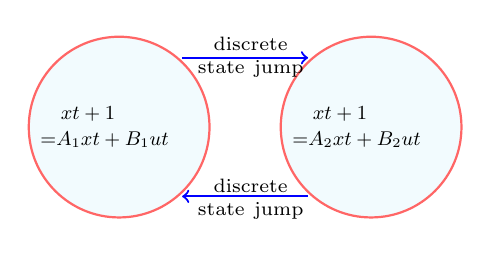
\begin{tikzpicture}[scale =0.8,
location/.style = {circle, draw=red!60, thick, fill = cyan!5}, ]


% Draw locations
\node[text width = 2.5 cm, scale =0.8, location] at (0,0) {{\small  \hspace{1em}$\trj{x}{t+1}$\\=$A_1\trj{x}{t}+B_1\trj{u}{t}$}};
\node[text width = 2.5 cm, scale =0.8, location] at (4,0) {{\small \hspace{1em}$\trj{x}{t+1}$\\=$A_2\trj{x}{t}+B_2\trj{u}{t}$}};

% Draw edges
\draw[thick, blue, ->,yshift=0.6cm] (1,0.5) --  (3,0.5);
\draw[thick, blue, <-,yshift=-0.6cm] (1,-0.5) --  (3,-0.5);

% Label edges
\node[text width = 1cm, yshift=0.5cm, xshift=0.1cm] at (2,0.7) {\scriptsize discrete};
\node[text width = 2cm, yshift=0.5cm, xshift=0.4cm] at (2,0.3) {\scriptsize state jump};
\node[text width = 1cm, yshift=-0.5cm, xshift=0.1cm] at (2,-0.3) {\scriptsize discrete };
\node[text width = 2cm, yshift=-0.5cm, xshift=0.4cm] at (2,-0.7) {\scriptsize state jump};

\end{tikzpicture}\\[0.5em]
%
$x\in\reals^n$: Continuous state\\
$l\in\set{l_1,...,l_k}$: Discrete state
\end{minipage}

\begin{minipage}{0.45\textwidth}
\begin{figure}
\center
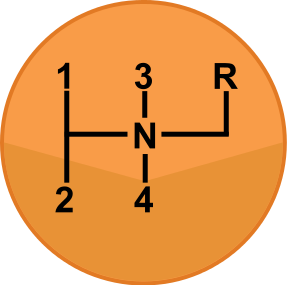
\includegraphics[width = 3cm, height = 3cm]{figures/downloaded/CarGear.png}
\caption{\small Gear control to switch dynamics}
\end{figure}
\end{minipage}
%
\begin{minipage}{0.45\textwidth}
\begin{figure}

\includegraphics[height = 3cm, width = 2.5cm]{figures/downloaded/ComputerControl.jpg}
\caption{\small Computer Controlled System}
\end{figure}
\end{minipage}

\end{frame}


%=========================================================================================================================================

\begin{frame}{Verification of Hybrid Systems is Challenging}
%
\begin{itemize}
\item Computing \negemph{exact set} of \negemph{reachable states} of hybrid systems  can be \negemph{computationally expensive} and \negemph{generally impossible}
\item Consider a simple \negemph{   affine switched system}:
\[
x(t+1) = A_ix(t)+u_i,~~i\in\set{1,2}.
\]
%
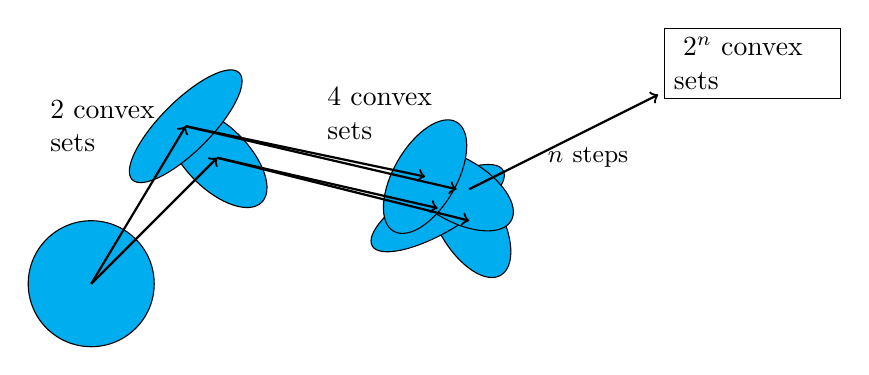
\begin{tikzpicture}[scale = 0.8
]
\draw[fill=cyan] (0,0) circle (1cm);

\draw[rotate around = {45:(2,2)}, fill=cyan] (2,2) ellipse (0.5cm and 1cm);
\draw[rotate around = {135:(1.5,2.5)}, fill=cyan] (1.5,2.5) ellipse (0.4cm and 1.2cm);
\draw[->,thick] (0,0) -- (2,2);
\draw[->,thick] (0,0) -- (1.5,2.5);
\node[text width = 2cm] at (0.6, 2.5) {$2$ convex\\ sets};

\draw[rotate around = {30:(6,1)}, fill=cyan] (6,1) ellipse (0.5cm and 1cm);
\draw[rotate around = {120:(5.5,1.2)}, fill=cyan] (5.5,1.2) ellipse (0.4cm and 1.2cm);
\draw[rotate around = {60:(5.8,1.5)}, fill=cyan] (5.8,1.5) ellipse (0.5cm and 1cm);
\draw[rotate around = {150:(5.3,1.7)}, fill=cyan] (5.3,1.7) ellipse (0.5cm and 1cm);
\draw[->,thick] (2,2) -- (6,1);
\draw[->,thick] (2,2) -- (5.5,1.2);
\draw[->,thick] (1.5,2.5) -- (5.3,1.7);
\draw[->,thick] (1.5,2.5) -- (5.8,1.5);
\node[text width = 2cm] at (5, 2.7) {$4$ convex \\sets};

\draw[->,thick] (6,1.5) -- (9,3);
\node[text width = 2cm] at (8.5,2) {\small $n$ steps};
\node[draw,text  width = 2cm]  at (10.5,3.5) {\negemph{ $2^n$ convex\\ sets}};
\end{tikzpicture}
%
\end{itemize}
%
\end{frame}

%==========================================================================================================================

\begin{frame}{Set Representation for Verification}
%To deal with \negemph{ undecidability} or \negemph{ high computational complexity} of representing reachable sets:
%
Need for set representations:
\begin{itemize}
\item To \plemph{efficiently} handle set of \plemph{possibly infinite solutions} arising from \plemph{non-determinism} in dynamics
\end{itemize}
%
\plemph{ Set Representation}:  A \posemph{ digital encoding} of a possibly infinite \posemph{ set of states}
%
\begin{minipage}{0.35\textwidth}
% Polytopic approximation of reachable set
\center{
\begin{tikzpicture}[scale=0.9]
\draw[rotate around = {30:(6,1)}, fill=cyan!30] (6,1) ellipse (0.5cm and 1cm);
\draw[rotate around = {120:(5.5,1.2)}, fill=cyan] (5.5,1.2) ellipse (0.4cm and 1.2cm);
\draw[rotate around = {60:(5.8,1.5)}, fill=cyan] (5.8,1.5) ellipse (0.5cm and 1cm);
\draw[rotate around = {150:(5.3,1.7)}, fill=cyan] (5.3,1.7) ellipse (0.5cm and 1cm);
% draw lines of polytope around above image
\draw[very thick,color=onyx] (4.38,0.53)--(5,2.7);
\draw[very thick,color=onyx] (5,2.7)--(5.8,2.6);
\draw[very thick,color=onyx] (5.8,2.6)--(6.6,1.75);
\draw[very thick,color=onyx] (6.6,1.75)--(6.8,0.9);
\draw[very thick,color=onyx] (6.8,0.9)--(6.575,0);
\draw[very thick,color=onyx] (6.575,0)--(4.38,0.53);
\end{tikzpicture}
}
%
\begin{exampleblock}{Polytopes}
\eqnemph{$\set{x:Tx\leq d, x\in\reals^n}$}\\
{\small \eqnemph{$T$}: real matrix, \eqnemph{${d}$}: vector of bounds.}
\end{exampleblock}
%
\end{minipage}
%
\hspace{2.5em}
\begin{minipage}{0.4\textwidth}
%
\vspace{-0.5em}
\centering{
%
\begin{tikzpicture}[scale=0.8]x
\draw[rotate around = {30:(6,1)}, fill=cyan] (6,1) ellipse (0.5cm and 1cm);
\draw[rotate around = {120:(5.5,1.2)}, fill=cyan] (5.5,1.2) ellipse (0.4cm and 1.2cm);
\draw[rotate around = {60:(5.8,1.5)}, fill=cyan] (5.8,1.5) ellipse (0.5cm and 1cm);
\draw[rotate around = {150:(5.3,1.7)}, fill=cyan] (5.3,1.7) ellipse (0.5cm and 1cm);
% draw ellipse around the above image
\draw[color=onyx, very thick, rotate around={70:(5.7,1.1)}] (5.7,1.1) ellipse (1.65cm and 1.225cm);
%
\end{tikzpicture}
%
}
%
\hspace{0.5em}
\begin{exampleblock}{Ellipsoid}
\eqnemph{$\set{x: (x-c)^TP(x-c)\leq 1}$}.\\
{\small \eqnemph{$P$}: Positive semi-definite matrix, \eqnemph{$c$}: real vector (center)}
\end{exampleblock}
%
\end{minipage}
%
\end{frame}

%====================================================================================================================================

%% \begin{frame}{Positive Invariant for Unbounded Time
%% Over-approximation}
%% Typically use \plemph{Positive Invariant} (PI) to approximate reachable
%% set for \posemph{unbounded/all time/s}.
%% %
%% \begin{block}{}
%% \center{Positive Invariant $\Psi$: \eqnemph{$\forall x\in\Psi, \operatorname*{Next}(x)\in\Psi$}.}
%% \end{block}
%% %
%% \begin{itemize}
%% \item \center{\eqnemph{
%% ({ {Initial~Set}$\subseteq$ PI)$\implies$ (Unbounded(t) 
%% reach set $\subseteq$ PI).}
%% }}
%% \end{itemize}
%% %
%% %\begin{minipage}{0.35\textwidth}
%% \center{
%% \begin{tikzpicture}[scale=2.5]
%% \draw[fill=cyan] plot[smooth cycle] coordinates {(0,0) (0.5,1)
%% (1,1.2) (1.5,0.9) (1.2,0) };
%% \draw[fill=red!30] plot[smooth cycle] coordinates {(0.2,0.2) (0.5,0.8)
%% (1,1) (1.5,0.8) (1.2,0.2) };
%% \draw[->,thick] (0,0)--(0.2,0.2);
%% \draw[->,thick] (0.5,1)--(0.5,0.8);
%% \draw[->,thick] (1,1.2)--(1,1);
%% \draw[->,thick] (1.5,0.9) -- (1.48,0.79);
%% \draw[->,thick] (1.2,0)--(1.2,0.2);
%% \draw[fill=white] (0.5,0) rectangle (1,0.5);
%% \node[text width = 0.25cm] at (0.75, 0.25) {\small Init.\\ Set };
%% %
%% \node at (1.8,0.6) {$\bm{\implies}$};
%% %
%% \draw[fill=cyan,xshift=2cm] plot[smooth cycle] coordinates {(0,0) (0.5,1)
%% (1,1.2) (1.5,0.9) (1.2,0) };
%% \draw[fill=yellow, rotate around={180:(2.75,0.4)}, xshift=1.85cm,yshift=-0.15cm] plot[smooth cycle] coordinates {(0.2,0.2) (0.5,0.8)
%% (1,1) (1.5,0.8) (1.2,0.2) };
%% \node[text width = 0.25cm,xshift=4.5cm,yshift=0.2cm] at (0.75, 0.25) { Reachable\\ Set };
%% \end{tikzpicture}
%% }
%% %\end{minipage}
%% %
%% \end{frame}

%=====================================================================================================================================

\begin{frame}{Requirements of a Set Representation}
%
Goal: \plemph{design set representation} for \plemph{efficiently computing} reachable states
%
%% \begin{enumerate}
%% \item \plemph{Reachability computation} for safety verification
%% \item \plemph{Positive invariant} computation
%% \item \plemph{Stability verification}
%% \end{enumerate}
%

\bigskip
Typically required operations:\\
\plemph{Linear transformation} (e.g. continuous dynamics), \plemph{Minkowski sum} (e.g. input disturbance), \plemph{Intersection with half-spaces} (e.g. switching dynamics), e.t.c
%
\vspace{2em}
\begin{itemize}
\item \posemph{Accurate} and \posemph{fast computation}: 
%\begin{enumerate}
 \plemph{closure} and \plemph{low computational complexity} under required set operations.
%% \begin{align*}
%% & \text{if}~T_{\trj{l}{t}}\trj{x}{t}\leq 1,~~ \trj{l}{t+1}=f(\trj{l}{t})\\
%% & \trj{x}{t+1}=
%% A_{\trj{l}{t}}\trj{x}{t}+\trj{u}{t}.
%% \end{align*}
%% }
%% %
%\end{enumerate}
\vspace{1em}

%Common set representations: \plemph{Polytopes, Ellipsoids, Zonotopes}
\end{itemize}
\end{frame}

%=================================================================================================================================

\begin{frame}{Plan}
%
\begin{enumerate}
\item  \plemph{Dynamics} of \plemph{embedded/cyber-physical} systems %\vspace{-1em}
%
%% \begin{itemize}
%% \item \plemph{hybrid system} models, \plemph{trajectory set computation}
%% \end{itemize}
%% %
\emph{}
%
\begin{block}{}
\item \plemph{Usual zonotope} $\rightarrow$ \plemph{complex zonotope}
%
\begin{itemize}
\item Capture \plemph{contraction} along \plemph{complex eigenvectors}
\end{itemize}
\end{block}
%
\emph{}
%
\item \plemph{Complex Zonotope} $\rightarrow$ \plemph{template complex zonotope}
%% \begin{itemize}
%% \item Motivation: \plemph{better approximation} of reachable sets
%% \item Basic \posemph{operations}: linear transformation, Minkowski sum, support function
%% \item \plemph{Checking inclusion} : \posemph{convex program}
%% \end{itemize}
%
\emph{}
%
\item \plemph{Template Complex Zonotope} $\rightarrow$ \plemph{Augmented complex zonotope}
%
%% \begin{itemize}
%% \item \posemph{Intersection} with \posemph{linear constraints}
%% \end{itemize}
%
\emph{}
%
\begin{alertblock}{}
\item \plemph{Applications}:
%
\begin{itemize}
\item \posemph{Stability verification} of \plemph{networked control} systems
%\item \posemph{Computing positive invariants} of discrete time affine hybrid systems
\item \posemph{Verification of linear invariance property} of  affine hybrid systems
\end{itemize}
\end{alertblock}
%
\end{enumerate}
%
\end{frame}

\section{Complex Zonotope}

%==================================================================================================================================

%% \begin{frame}{Review of Some Set Representations}
%% %
%% \begin{itemize}
%% \item Polytopes: \eqnemph{$Tx\leq d$} where $T$: real matrix, $d$: vector of bounds

%% \end{itemize}
%% %
%% \end{frame}

%% %% \begin{frame}{Features of Polytopes and Ellipsoids}
%% %% %
%% %% \begin{minipage}{0.48\textwidth}
%% %% \underline{\plemph{Polytope}}:
%% %% \begin{enumerate}
%% %% \item \emph{Linear transformation}: \posemph{Efficient} for \posemph{invertible matrix};
%% %% \negemph{Otherwise Exponential Complexity}.
%% %% \item \emph{Minkowski sum}: More than \negemph{Exponential
%% %% Complexity}.
%% %% \item \emph{Positive Invariant}: \posemph{Exists} for stable linear
%% %% transformation, but \negemph{compleixty of encoding} is \negemph{unbounded}.
%% %% \end{enumerate}
%% %% \end{minipage}
%% %% %
%% %% \begin{minipage}{0.48\textwidth}
%% %% \vspace{-3em}
%% %% \underline{\plemph{Ellipsoid}}:
%% %% %
%% %% \begin{enumerate}
%% %% \item \emph{Invertible Linear transformation} is \posemph{efficiently
%% %% computable}.
%% %% \item \emph{Minkowski sum}: \negemph{Not closed}.
%% %% \item \emph{Positive Invariant}: \posemph{Exists}
%% %% and \posemph{Efficiently encodable} for stable linear transformation.
%% %% \end{enumerate}
%% %% %
%% %% \end{minipage}
%% %% %
%% %% \end{frame}

%==================================================================================================================================

\begin{frame}{Usual Zonotope}
A \plemph{zonotope} is a \plemph{projection} of \plemph{higher dimensional hypercube}
onto \plemph{lower dimensional} space.\\[0.5em]
%
We consider a real matrix of \eqnemph{generators $V$} and \eqnemph{center $c$}
 %
\begin{block}{}
\center{
\eqnemph{
$
\rztope{\ptemp}{\cen}:=\set{\cen+\ptemp\zeta:~\zeta\in[-1,1]^m}.
$
}
}
%
\end{block}
%
\vspace{0.5em}
%
\begin{minipage}{0.43\textwidth}
{\scriptsize $V=\mymatrix{1 &   -1 &          0 &    0.5 \\
   -1 &         0 &   -1 &    0.5}$}
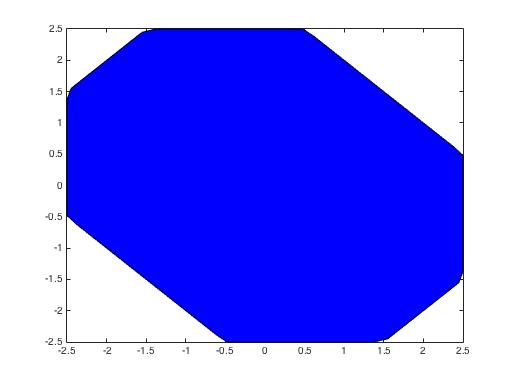
\includegraphics[scale=0.25]{figures/CZtopes/RealZonotope.jpg}
\end{minipage}
%
%\emph{}
\vline
%
\begin{minipage}{0.55\textwidth}
\begin{enumerate}
\item \posemph{Linear transformation} and \posemph{Minkowski sum}: Simple \posemph{algebraic} expressions
\item \posemph{Advantage} over \negemph{polytope} and \negemph{ellipsoid}
%
%% \eqnemph{\[
%% A\rztope{\ptemp}{\cen}=\rztope{A\ptemp}{A\cen}.
%% \]}
%
%\vspace{-2em}
%\item \posemph{Advantage} over \posemph{ellipsoid}:  \posemph{Efficient Minkowski sum}
%
%% \eqnemph{\begin{align*}
%% & \rztope{\ptemp}{\cen}\oplus\rztope{\ptemp^\pr}{\cen^\pr}\\
%% & = \rztope{\mymatrix{\ptemp & \ptemp^\pr}}{\cen+\cen^\pr}.  
%% \end{align*}}
%% %
\end{enumerate}
%
\end{minipage}
%
\end{frame}

%==================================================================================================================================


\begin{frame}{Drawback of Zonotopes for Computing Positive Invariants}
%
\begin{minipage}{0.48\textwidth}
\plemph{Positive Invariant}: \plemph{Next} reachable set \plemph{contained inside} the original set.
%
{\small
\begin{itemize}
\item \negemph{Directions for convergence} to an \negemph{equilibrium} can be
encoded by \negemph{complex valued eigenvectors}.
\item Usual \negemph{zonotopes} only have
\negemph{real eigenvectors} as \negemph{generators}.
\end{itemize}
}
%
\end{minipage}
%
\begin{minipage}{0.48\textwidth}

\center{
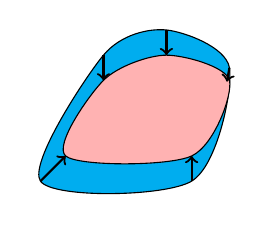
\begin{tikzpicture}[scale=1.6]
\draw[fill=cyan] plot[smooth cycle] coordinates {(0,0) (0.5,1)
(1,1.2) (1.5,0.9) (1.2,0) };
\draw[fill=red!30] plot[smooth cycle] coordinates {(0.2,0.2) (0.5,0.8)
(1,1) (1.5,0.8) (1.2,0.2) };
\draw[->,thick] (0,0)--(0.2,0.2);
\draw[->,thick] (0.5,1)--(0.5,0.8);
\draw[->,thick] (1,1.2)--(1,1);
\draw[->,thick] (1.5,0.9) -- (1.48,0.79);
\draw[->,thick] (1.2,0)--(1.2,0.2);
\end{tikzpicture}
}
%
\begin{figure}
\caption{$a+\iota b:~a\neq 0~~b\neq 0$.}
\vspace{-1em}
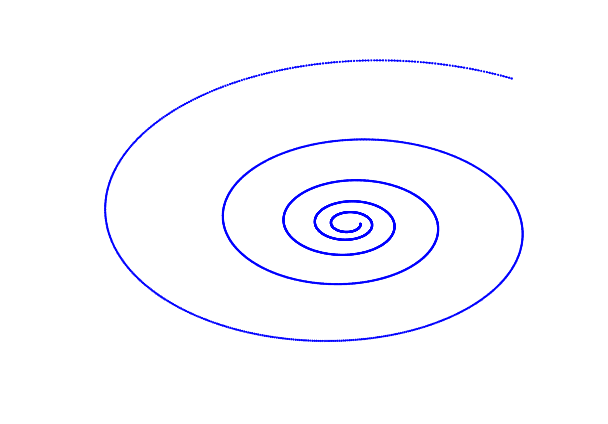
\includegraphics[scale=0.15]{figures/CZtopes/InwardSpiral.png}
\end{figure}
\end{minipage}
%
\emph{}
%
\begin{block}{}
{\small
Let us consider  a \plemph{stable real matrix} \eqnemph{$A$} whose \plemph{real
eigenvalues} are \eqnemph{$\mu$} and  \plemph{eigenvectors} are \eqnemph{$\ptemp$}.%, i.e., \eqnemph{$A\ptemp = \ptemp\diagonal{\mu}$}.
}
Then\hspace{1em} {\eqnemph{
$A\lt(\rztope{\ptemp}{0}\rt)\subseteq \rztope{\ptemp}{0}$% \plemph{(inclusion after transformation)}
}}
\end{block}
%
\negemph{*} We \negemph{can not rely} on above proposition when \negemph{eigenvectors are complex}.
\end{frame}

%==================================================================================================================================

\begin{frame}{Complex Zonotope: A New Set Representation}

{\small
\begin{itemize}
\item Extend \posemph{simple zonotope to complex numbers} in a way that can \posemph{capture
contraction along complex vectors}.
\item \plemph{Complex valued generators} with \plemph{Complex combining
coefficients} whose \plemph{absolute value $<=1$}.
\item Geometrically, \plemph{Minkowski sum} of \plemph{Ellipses}
and \plemph{Line Segments}.
\end{itemize}
%
Let us consider a  \plemph{complex} matrix $\ptemp$ and  a real vector (center) $\cen$.
}
%
\begin{block}{}
\center{
\eqnemph{$
\cztope{\ptemp}{\cen} := \set{\ptemp\zeta+\cen:~\zeta\in\compnums^m,~\infnorm{\zeta}\leq 1}.
$}
}
\end{block}
%
\begin{minipage}{0.35\textwidth}
%
\begin{tikzpicture}[scale=1]
\node[text width = 1cm] at (0,2) {{\small $\mymatrix{1+2\iota\\1-2\iota}$}};
\draw[thick,fill=cyan, rotate around = {135:(0,0)}] (0,0) ellipse
(1cm and 0.5cm);
\draw[->] (0,1.5)--(0,0.8);
\node at (1.5,1){$\bigoplus$};
\end{tikzpicture}
%
\end{minipage}
%
\begin{minipage}{0.3\textwidth}
%
\begin{tikzpicture}[scale=0.8]
\node[text width = 1cm] at (0,3.5) {{\small $\mymatrix{1\\1}$}};
\draw[color=blue,very thick] (-0.5,0.5)--(1,2);
\draw[->] (-0.2,3)--(-0.2,1.5);
\node at (1.5,2.5){$\bigoplus$};
\end{tikzpicture}
%
\end{minipage}
%
\begin{minipage}{0.3\textwidth}
%
\begin{tikzpicture}[scale=1]
\node[text width = 1cm] at (0,2) {{\small$\mymatrix{2+\iota\\2-\iota}$}};
\draw[thick,fill=cyan, rotate around = {45:(0,0)}] (0,0) ellipse
(1cm and 0.5cm);
\draw[->] (0,1.5)--(0,0.8);
\end{tikzpicture}
%
\end{minipage}
%
\end{frame}

%==================================================================================================================================

\begin{frame}{Non-polytopic Projection of Complex Zonotope}
%
\begin{figure}
\center
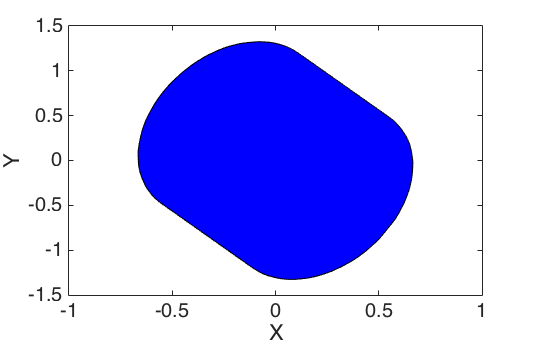
\includegraphics[scale=0.3]{figures/CZtopes/xycz.png}
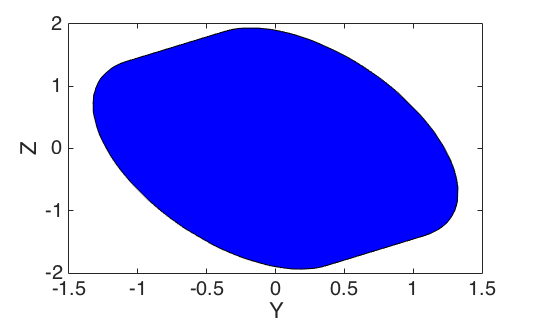
\includegraphics[scale=0.3]{figures/CZtopes/yzcz.png}\\
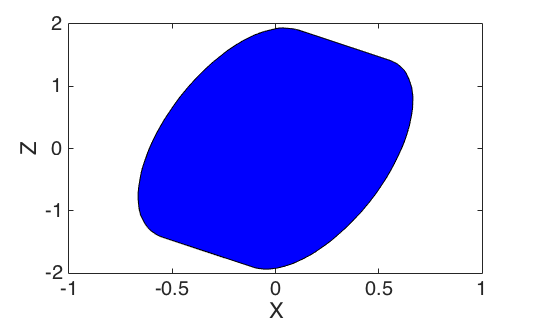
\includegraphics[scale=0.3]{figures/CZtopes/xzcz.png}
%\caption{Real projection of complex zonotope on axis oriented hyperplanes}~\label{fig:3dcztope}
\end{figure}
%
\end{frame}

%==================================================================================================================================

\begin{frame}{Complex Zonotopes: Ability to Capture Contraction along Complex Eigenvectors}

\begin{block}{}
{\small
Let \plemph{$A$} be a stable matrix having \plemph{complex eigenvalues} $\mu$ and \plemph{complex eigenvectors} $\ptemp$
}
%\begin{enumerate}
\center{\eqnemph{
%\item $A\lt(\cztope{\ptemp}{0}\rt)
%= \cztope{\ptemp\diagonal{{\mu}}}{0}.$
%\item If
%$\infnorm{\mu}\leq 1$, then
$A\lt(\cztope{\ptemp}{0}\rt)\subseteq \cztope{\ptemp}{0}$.
}
}
%\end{enumerate}
%
\end{block}
%
\begin{figure}
\center
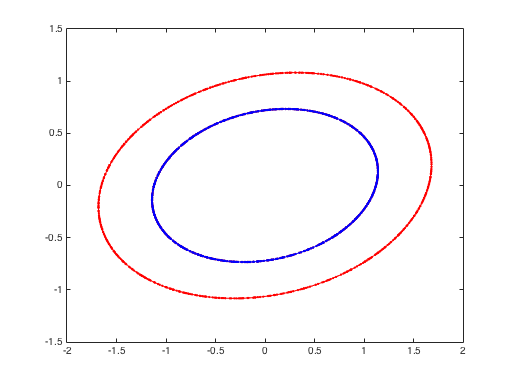
\includegraphics[scale=0.25]{figures/CZtopes/eigcontraction.png}\\
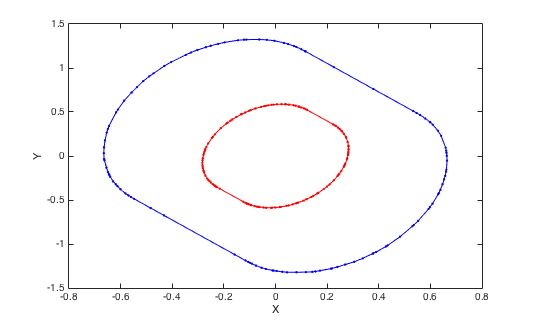
\includegraphics[scale=0.25]{figures/CZtopes/contraction-zonotope.png}
%\caption{Contraction of complex zonotope along
%eigenvectors}~\label{fig:cz-scaled-down}
\end{figure}
%
\end{frame}

%==================================================================================================================================



%==================================================================================================================================
\begin{frame}{Plan}
%
\begin{enumerate}
\item  \plemph{Dynamics} of \plemph{embedded/cyber-physical} systems %\vspace{-1em}
%
%% \begin{itemize}
%% \item \plemph{hybrid system} models, \plemph{trajectory set computation}
%% \end{itemize}
%% %
\emph{}
%
\item \plemph{Usual zonotope} $\rightarrow$ \plemph{Complex zonotope}
%
%% \begin{itemize}
%% \item Capture \plemph{contraction} along \plemph{complex eigenvectors}
%% \end{itemize}
%
\emph{}
%
\begin{block}{}
\item \plemph{Complex zonotope} $\rightarrow$ \plemph{Template complex zonotope}
\begin{itemize}
\item Motivation: \plemph{better approximation} of reachable sets
\item Basic \posemph{operations}: linear transformation, Minkowski sum, support function
\item \plemph{Checking inclusion} : \posemph{convex program}
\end{itemize}
\end{block}
%
\emph{}
%
\item \plemph{Template Complex Zonotope} $\rightarrow$ \plemph{Augmented complex zonotope}
%
%% \begin{itemize}
%% \item \posemph{Intersection} with \posemph{linear constraints}
%% \end{itemize}
%
\emph{}
%
\begin{alertblock}{}
\item \plemph{Applications}:
%
\begin{itemize}
\item \posemph{Stability verification} of \plemph{networked control} systems
%\item \posemph{Computing positive invariants} of discrete time affine hybrid systems
\item \posemph{Verification of linear invariance property} of   affine hybrid systems
\end{itemize}
\end{alertblock}
%
\end{enumerate}
%
\end{frame}

\section{Template complex zonotope}

%==================================================================================================================================

%% \begin{frame}{Template Complex Zonotope: Motivation}

%% Problem with \negemph{refining} a        complex zonotope\\[1em]

%% \negemph{*} \negemph{Better approximation} by complex
%% zonotope \negemph{can not} be found by \negemph{adding generator}.
%% %
%% \begin{enumerate}
%% \item \negemph{Increases size}.
%% \item \negemph{Distorts positive invariance}.
%% \end{enumerate}
%% %
%% \begin{figure}
%% \center
%% 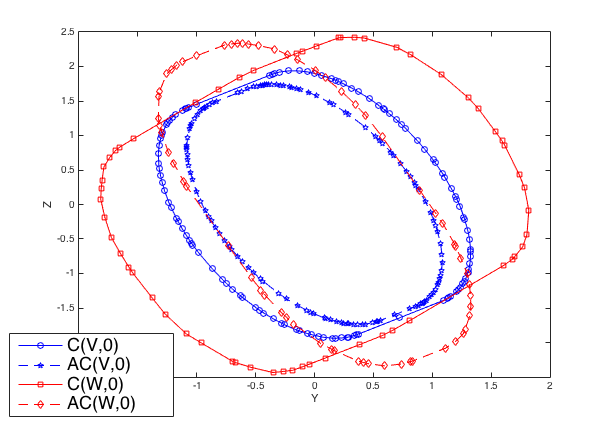
\includegraphics[scale=0.3]{figures/CZtopes/refinement.png}
%% %% \caption{Violation of positive invariance and size increase after
%% %% adding a generator to the basic representation.}~\label{fig:refinement}
%% \end{figure}
%% %
%% \end{frame}


%==================================================================================================================================

\begin{frame}{Template Complex Zonotope: Definition}
\plemph{Variable bounds} on absolute values of \plemph{combining
coefficients}.\\[0.5em]

{\small
${\ptemp\in\mat{n}{m}{\compnums}}$: \plemph{template},
\fbox{${\sfact\in\reals^m_{\geq 0}}$: \plemph{scaling factors}},
${\cen\in\reals^n}$: \plemph{center}.
}
%
\begin{block}{}
%
\center{\eqnemph{
$
\tcztope{\ptemp}{\cen}{\sfact}
= \set{\ptemp\zeta+\cen:~\absolute{\zeta_i}\leq \sfact_i~\forall
i\in\set{1,...,m}}.
$
}}
\end{block}
%
\begin{itemize}
\item \posemph{Add more generators} and \posemph{adjust scaling} factors to find \posemph{better approximations}.
\end{itemize}
%
\begin{tikzpicture}[scale=2.5]
\draw[fill = orange] plot[smooth cycle] coordinates{(0,-0.2) (-0.7,0.5) (0,1) (1,0.75) (1,0) (0.5,-0.5)};
\draw[fill = green] plot[smooth cycle] coordinates{(0,0) (-0.5,0.5) (0,1) (0.75,0.75) (1,0) (0.5,-0.25)};
\draw[fill = blue] plot[smooth cycle] coordinates{(0,0) (-0.25,0.5) (0,1) (0.75,0.4) (1,0) (0.5,-0.1) };
\draw[fill=yellow] (0,0)--(0,1)--(1,0)--cycle;
\draw[->] (0.6,0.75)--(1.75,0.75);
\node at (2.25,0.75) {$\cztope{V}{c}$};
\draw[->] (0.68,0.4)--(1.4,0.4);
\node  at (2.25,0.4) {$\tcztope{\mymatrix{V & W}}{c}{\mymatrix{a\\b}}$};
\draw[->] (0.5,-0.4)--(1.7,-0.1);
\node at (2.25,0) {$\cztope{\mymatrix{V & W}}{s}$};
\draw[very thick,dashed,->] (0,0)--(-0.3,-0.3);
\node at (-0.4,-0.4) {$W$};
\end{tikzpicture}
%
\end{frame}

%==================================================================================================================================

\begin{frame}{Basic Operations: Template Complex Zonotope}
%
\begin{enumerate}
\eqnemph{
\item
$A\tcztope{\ptemp}{\cen}{\sfact}=\tcztope{A\ptemp}{A\cen}{\sfact}$.
\item $\minsum{\tcztope{\ptemp}{\cen}{\sfact}}{\tcztope{\ptemp^\pr}{\cen^\pr}{\sfact^\pr}}
= \tcztope{\begin{bmatrix}\ptemp
& \ptemp^\pr\end{bmatrix}}{\cen+\cen^\pr}{\begin{bmatrix}\sfact\\\sfact^\pr\end{bmatrix}}$.
}
%% \item {\small Let $\supp{v}{\Psi}=\sup_{x\in\Psi}v^Tx$}. Then \plemph{support
%% function}\\
%% \eqnemph{
%% \[
%% \supp{v}{\real\lt(\tcztope{\ptemp}{\cen}{\sfact}\rt)}=v^Tc+\absolute{v^T\ptemp}\sfact.
%% \]
%% }
\end{enumerate}
%
\begin{itemize}
\item Above are \posemph{affine functions} of \posemph{center}
and \posemph{scaling factors}.
\end{itemize}
%
\end{frame}


%==================================================================================================================================

\begin{frame}{Checking Inclusion}
Generally, checking inclusion between complex zonotopes requires \negemph{non-convex
optimization}.
But we propose a \posemph{convex relaxation} that  \posemph{works well
in practice}.\\[0.5em]
%
{\small 
%
\begin{definition}[\eqnemph{$\tcztope{\ptemp^\pr}{\cen^\pr}{\sfact^\pr}\order\tcztope{\ptemp}{\cen}{\sfact}$}]
%
\vspace{-1em}
\begin{align*}
& \exists \tmat\in\mat{m}{r}{\compnums},\tvect\in\compnums^m~~\text{such
that}\\
& \ptemp\tmat=\ptemp^\pr\diagonal{\sfact^\pr},~~\ptemp\tvect=\cen^\pr-\cen~\\%\numberthis\label{eqn:inclusion-tcz1}\\
& \max_{i=1}^m\lt(\absolute{\tvect_i}+\sum_{j=1}^r\absolute{\tmat_{ij}}-\sfact_i\rt)\leq
0.
\end{align*}
%
\end{definition}
}
\vspace{0.3em}
\begin{minipage}{0.37\textwidth}
\begin{exampleblock}{}
\center{\eqnemph{Result: 
$\order\implies\subseteq$.
}}
\end{exampleblock}
\end{minipage}
%
\begin{minipage}{0.6\textwidth}
\begin{itemize}
\item $\order$: \plemph{Second order conic constraints} (convex
constraints) on \plemph{center} and \plemph{scaling factors}.
\end{itemize}
\end{minipage}
%
\end{frame}

%==================================================================================================================================

\begin{frame}{Intersection between Complex Zonotopes}
%
\begin{itemize}
\item Closed for \plemph{common invertible template}
\end{itemize}
%
\begin{block}{}
Let us consider a \plemph{invertible} matrix $\ptemp$
%

\begin{center}
\eqnemph{
$\tcztope{\ptemp}{\cen}{\sfact}\bigcap\tcztope{\ptemp}{\cen}{\sfact^\pr}=\tcztope{\ptemp}{\cen}{\meet{\sfact}{\sfact^\pr}}$.
}
\end{center}
%
\end{block}
%
\begin{minipage}{0.48\textwidth}
\begin{figure}
  \center
  \caption{Non-closure  for a non-invertible template.}
  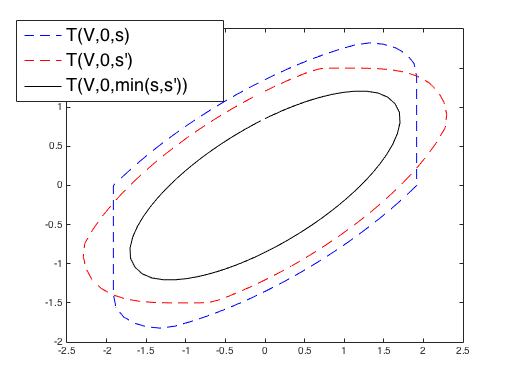
\includegraphics[scale=0.3]{figures/CZtopes/nonclosure.png}
\end{figure}
\end{minipage}
%
\begin{minipage}{0.48\textwidth}
\begin{figure}
  \center
  \caption{Closure for an invertible template.}
  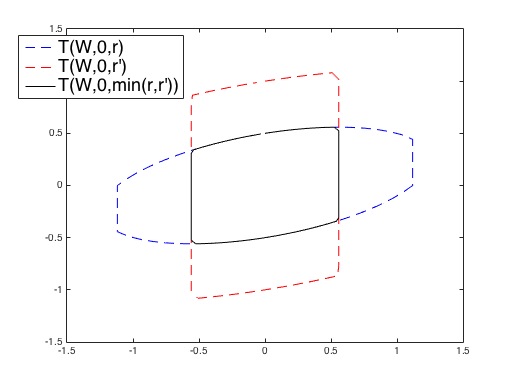
\includegraphics[scale=0.35]{figures/CZtopes/closure.png}
\end{figure}
\end{minipage}
%
\end{frame}

%==================================================================================================================================

\begin{frame}{Comparison with Existing Set Representations}
%
\begin{table}
\resizebox{\textwidth}{!}{
\begin{tabular}{|l|c|c|c|c|}
\hline
\multirow{2}{*}{Set} & \multirow{2}{*}{Linear} & \multirow{2}{*}{Minkowski} & \multirow{2}{*}{Intersection } & {Positive Invariant }\\
\multirow{2}{*}{representation} & \multirow{2}{*}{transformation} & \multirow{2}{*}{sum} & \multirow{2}{*}{with half-space} & (non-empty interior)\\
& & & & stable invertible\\
& & & & linear transformation\\
\hline
\multirow{2}{*}{Convex polytope} & {\negemph{Efficient} } & \negemph{More than}
& \multirow{3}{*}{\posemph{Efficient}}  &  \negemph{Maximum complexity}\\
\multirow{2}{*}{$H$-representation} & \negemph{only for} & \negemph{exponential}  &  & \negemph{of encoding}  \\
& \negemph{invertible matrix} & \negemph{complexity} & & \negemph{not bounded} \\
\hline
\multirow{2}{*}{Zonotope} & \multirow{2}{*}{\posemph{Efficient}}
& \multirow{2}{*}{\posemph{Efficient}} & \negemph{Not} & \negemph{May not}\\
& & & \negemph{closed} & \negemph{exist}\\
\hline
\multirow{2}{*}{Ellipsoid} & \multirow{2}{*}{\posemph{Efficient}} & \negemph{Not} & \negemph{Not} &
\posemph{Efficient}\\
& & \negemph{closed} & \negemph{closed} & \posemph{encoding}\\
\hline
\multirow{2}{*}{Polynomial} & \negemph{More than} & \negemph{More than} & \multirow{3}{*}{\posemph{Efficient}} &
\multirow{2}{*}{\posemph{Efficient}} \\
\multirow{2}{*}{sub-level set} & \negemph{exponential} & \negemph{exponential} &
& \multirow{2}{*}{\posemph{encoding}}\\
& \negemph{complexity} & \negemph{complexity} & & \\
\hline
\plemph{Template Complex} & \multirow{2}{*}{\posemph{Efficient}} & \multirow{2}{*}{\posemph{Efficient}} &
\negemph{Not} & \posemph{Efficient}\\
\plemph{Zonotope} & & & \negemph{closed} & \posemph{encoding}\\
\hline
\end{tabular}
}
%\caption{Comparison of set representations}~\label{tab:compset}
\end{table}
%
\end{frame}

%==================================================================================================================================

\begin{frame}{Plan}
%
\begin{enumerate}
\item  \plemph{Dynamics} of \plemph{embedded/cyber-physical} systems %\vspace{-1em}
%
%% \begin{itemize}
%% \item \plemph{hybrid system} models, \plemph{trajectory set computation}
%% \end{itemize}
%% %
\emph{}
%
\item \plemph{Usual zonotope} $\rightarrow$ \plemph{Complex zonotope}
%
%% \begin{itemize}
%% \item Capture \plemph{contraction} along \plemph{complex eigenvectors}
%% \end{itemize}
%
\emph{}
%
\item \plemph{Complex zonotope} $\rightarrow$ \plemph{Template complex zonotope}
%% \begin{itemize}
%% \item Motivation: \plemph{better approximation} of reachable sets
%% \item Basic \posemph{operations}: linear transformation, Minkowski sum, support function
%% \item \plemph{Checking inclusion} : \posemph{convex program}
%% \end{itemize}
%% %
%% \emph{}
%
\begin{block}{}
\item \plemph{Template Complex Zonotope} $\rightarrow$ \plemph{Augmented complex zonotope}
%
\begin{itemize}
\item \posemph{Intersection operation} for \posemph{discrete transitions}
\end{itemize}
\end{block}
%
\emph{}
%
\begin{alertblock}{}
\item \plemph{Applications}:
%
\begin{itemize}
\item \posemph{Stability verification} of \plemph{networked control} systems
%\item \posemph{Computing positive invariants} of discrete time affine hybrid systems
\item \posemph{Verification of linear invariance property} of   affine hybrid systems
\end{itemize}
\end{alertblock}
%
\end{enumerate}
%
\end{frame}

\section{Augmented complex zonotope}

%==================================================================================================================================

%\section{Operations on a Complex Zonotope}



%==================================================================================================================================

\begin{frame}{Augmented complex zonotope: Motivation}
%
To handle discrete transitions, we compute intersection with guards.  But intersection is \negemph{not closed}.\\[1.5em]
%
\begin{minipage}{1\textwidth}
{ Earlier \posemph{solutions}: extensions of \posemph{real zonotope} 

\begin{itemize}
\item \plemph{Constrained Zonotope}~\cite{scott2016constrained}, \plemph{Constrained Affine set}~\cite{Ghorbal2010}\\[0.5em]
\item Allow \plemph{additional linear constraints} on \plemph{coefficients}.
\item Using this idea for complex zonotopes is not tractable
\end{itemize}
%
}
\end{minipage}
\emph{}
%
%{\small
\vspace{1em}



$\Rightarrow$ Our solution: \plemph{Augmented complex zonotope}

%% \begin{minipage}{0.48\textwidth}
%% \eqnemph{\small
%% \begin{align*}
%% & \cztope{\mymatrix{1+2\iota & 2+\iota\\ 1-2\iota &2-\iota}}{0}
%% \bigcap\set{x: x\leq 0}\\[0.5em]
%% \hline\\[-1em]
%% &= \set{\begin{array}{c}
%% \mymatrix{1+2\iota & 2+\iota\\ 1-2\iota & 2-\iota}(\zeta+\iota\epsilon):\\
%% ~\\[-0.5em]
%% \hline
%% \multicolumn{1}{|c|}{\zeta_i^2+\epsilon_i^2\leq 1~\forall i\in\set{1,2}}\\
%% \hline
%% ~\\[-0.5em]
%% \hline
%% \multicolumn{1}{|c|}{\zeta_1+\zeta_2-2\epsilon_1+2\epsilon_2\leq 0}\\
%% \hline
%% \end{array}
%% }.
%% \end{align*}
%% }
%% \end{minipage}
%
%\begin{minipage}{0.45\textwidth}
%% \begin{itemize}
%% \item Computing \negemph{support function} becomes \negemph{intractable}.
%% \item \negemph{Can not} find \negemph{practically useful} convex relaxation for \negemph{inclusion-checking}.
%% \end{itemize}
%
%\end{minipage}
%
\end{frame}


%==================================================================================================================================




%==================================================================================================================================

\begin{frame}{Augmented Complex Zonotope : Definition}
%
\begin{minipage}{0.5\textwidth}
\begin{itemize}
%\item Some combining coefficients have \plemph{absolute value bounds} and others have \plemph{interval bounds}.
\item \plemph{Minkowski sum} of \plemph{template complex zonotope} and \plemph{interval zonotope}.
\end{itemize}
\end{minipage}
%
\vline\hspace{1em}
%
\begin{minipage}{0.44\textwidth}
%
{
\begin{exampleblock}{\center{Interval Zonotope: $\iztope{\stemp}{\lb}{\ub}$}}
\eqnemph{$\set{\stemp\zeta:~\zeta\in\reals^k,~\lb\leq\zeta\leq\ub}.$}
\end{exampleblock}
}
%
\begin{block}{Template Complex Zonotope\\ $\oplus$ Interval Zonotope}
\eqnemph{
$\minsum{\tcztope{\ptemp}{\cen}{\sfact}}{\iztope{\stemp}{\lb}{\ub}}$.
}
\end{block}
\end{minipage}

%
%% \begin{alertblock}{}
%% $\ptemp$: Primary template, $\cen$: primary offset, $\sfact$: scaling factors, $\stemp$: secondary template, $\lb$: lower interval bound, $\ub$: upper interval bound.
%% \end{alertblock}
%
\vspace{1em}
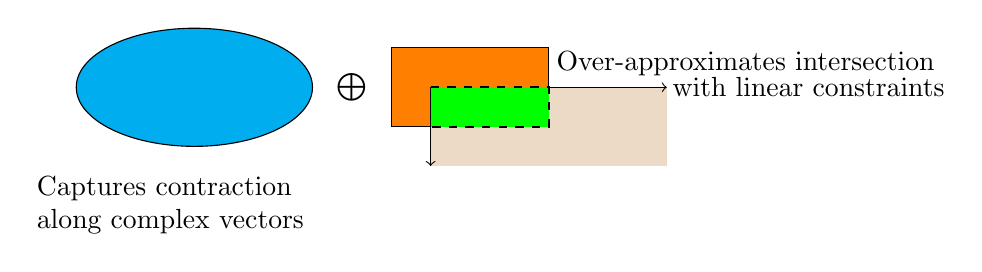
\begin{tikzpicture}[block/.style={rectangle, fill=magenta!60}]
\draw[fill=cyan] (0,0) ellipse (1.5cm and 0.75cm);
\node at (2,0) {$\bigoplus$};
\draw[fill=orange] (2.5,-0.5) rectangle (4.5,0.5);
\fill[brown!30] (3,0)--(6,0)--(6,-1)--(3,-1)--cycle;
\draw[->] (3,0)--(3,-1);
\draw[->] (3,0)--(6,0);
\draw[dashed,thick,fill=green] (3,0)--(4.5,0)--(4.5,-0.5)--(3,-0.5);
%\draw[->] (0,0)--(0,-1);
\node [text width = 4cm] at (0,-1.5) {Captures contraction\\along complex vectors};
\node at (7,0.3) {Over-approximates intersection};
\node at (7.8,0) {with linear constraints};
\end{tikzpicture}
\end{frame}

%==================================================================================================================================

%% \begin{frame}{Intersection with Minkowski sum}
%% %
%% \begin{minipage}{0.48\textwidth}
%% Let us consider set\\ \eqnemph{$S:~\forall i\in\set{1,...,k}$} and
%% %
%% \eqnemph{
%% \begin{block}{}
%% $\lt(\identity{n}{n}-\diagonal{\bm{e}_i}\rt)\qtemp S \subseteq \qtemp S$.
%% \end{block}
%% }
%% %
%% \end{minipage}
%% %
%% \begin{minipage}{0.48\textwidth}
%% %
%% \begin{center}
%% $\forall P\in \qtemp S$.
%% \begin{tikzpicture}[scale=1]
%% \coordinate (samplept) at (1.15,0.83);
%% \draw[fill=cyan] (0,0) ellipse (2cm and 1cm);
%% \fill[color=yellow] (0,0) rectangle (samplept);
%% \draw[dashed, thick, ->] (0,0)--(samplept);
%% \node at (1.17,1) {P};
%% \end{tikzpicture}
%% \end{center}
%% %
%% \end{minipage}
%% %
%% \emph{}
%% %
%% \begin{block}{Result}
%% \begin{itemize}
%% \eqnemph{
%% \item $\lt(\lt(S\oplus \iztope{\pinv{\qtemp}}{\lb}{\ub}\rt)\bigcap\ptope{\qtemp}{\plb}{\pub}\rt)
%% \subseteq \lt(S \oplus\iztope{\pinv{\qtemp}}{\join{\lb}{\plb}}{\meet{\ub}{\pub}}\rt).$
%% }
%% \item \plemph{Over-approximation error} positively correlated to \plemph{size of $\qtemp S$}.
%% \end{itemize}
%% \end{block}
%% %
%% \vspace{-1.5em}
%% %
%% \begin{center}
%% \begin{tikzpicture}[block/.style={rectangle, fill=magenta!60}]
%% \draw[fill=cyan] (0,0) ellipse (1.5cm and 0.75cm);
%% \node at (2,0) {$\bigoplus$};
%% \draw[fill=orange] (2.5,-0.5) rectangle (4.5,0.5);
%% \fill[brown!30] (3,0)--(6,0)--(6,-1)--(3,-1)--cycle;
%% \node at (5.5,-0.6) {$T$};
%% \draw[->] (3,0)--(3,-1);
%% \draw[->] (3,0)--(6,0);
%% \draw[dashed,thick,fill=green] (3,0)--(4.5,0)--(4.5,-0.5)--(3,-0.5);
%% \draw[->,thick] plot [smooth] coordinates{(0.8,0.5) (1.5,1) (3,0.5)};
%% \node at (1.5,1.3) {$\Psi_1$};
%% \draw[->,thick] plot [smooth] coordinates{(0.8,-0.5) (1.5,-1) (3.5,-0.5)};
%% \node at (1.5,-1.3) {$\Psi_2$};
%% \node[block] at (8,0) {{\Large
%% $\lt(\Psi_1\bigcap T\rt)\subseteq\Psi_2$
%% }};
%% \end{tikzpicture}
%% \end{center}
%% %
%% \end{frame}

%==================================================================================================================================

\begin{frame}{Augmented Complex Zonotope: Intersection with Parallelotope}
%
\begin{minipage}{0.48\textwidth}
\begin{itemize}
\item \plemph{Parallelotope} $P$= \eqnemph{$\ptope{\qtemp}{\plb}{\pub}$}
\item \plemph{Template complex zonotope}\\ $S=\tcztope{V}{c}{s}$ s.t. \eqnemph{$\forall i\in\set{1,...,k}$}
\end{itemize}
%
%
\end{minipage}
%
%\hspace{2em}
%
\begin{minipage}{0.48\textwidth}
%
\center{
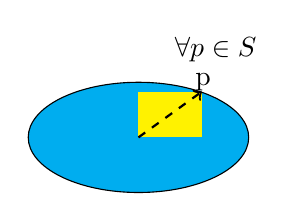
\begin{tikzpicture}[scale=0.7]
\coordinate (samplept) at (1.15,0.83);
\draw[fill=cyan] (0,0) ellipse (2cm and 1cm);
\fill[color=yellow] (0,0) rectangle (samplept);
\draw[dashed, thick, ->] (0,0)--(samplept);
\node at (1.17,1) {p};
\node at (1.4,1.6) {$\forall p\in \qtemp S$};
\end{tikzpicture}
}
%
\eqnemph{
\begin{exampleblock}{}
$\lt({Id}-\diagonal{\bm{e}_i}\rt)\tcztope{\qtemp\ptemp}{\qtemp\cen}{\sfact}$ $\order  \tcztope{\qtemp\ptemp}{\qtemp\cen}{\sfact}$.
\end{exampleblock}
}
\end{minipage}
%
\begin{block}{}
\begin{itemize}
\item \plemph{Augmented complex zonotope} \eqnemph{$\acztope{\ptemp}{\cen}{\sfact}{\pinv{\qtemp}}{\lb}{\ub}$} \plemph{constructed from} \eqnemph{$S$} and the parallelotope $P$ where
$\pinv{\qtemp}:$ Pseudo-inverse of $\qtemp$
\eqnemph{
\item $\acztope{\ptemp}{\cen}{\sfact}{\pinv{\qtemp}}{\lb}{\ub}\bigcap\ptope{\qtemp}{\plb}{\pub}
\subseteq \acztope{\ptemp}{\cen}{\sfact}{\pinv{\qtemp}}{\join{\lb}{\plb}}{\meet{\ub}{\pub}}$
}
\item \plemph{Over-approximation error} positively correlated to \plemph{magnitude of $\qtemp\ptemp$}
\end{itemize}
\end{block}
%
%\vspace{-1.5em}
%
%% \begin{center}
%% \begin{tikzpicture}[block/.style={rectangle, fill=magenta!60},scale=0.75]
%% \draw[fill=cyan] (0,0) ellipse (1.5cm and 0.75cm);
%% \node at (2,0) {$\bigoplus$};
%% \draw[fill=orange] (2.5,-0.5) rectangle (4.5,0.5);
%% \fill[brown!30] (3,0)--(6,0)--(6,-1)--(3,-1)--cycle;
%% \node at (5.5,-0.6) {$T$};
%% \draw[->] (3,0)--(3,-1);
%% \draw[->] (3,0)--(6,0);
%% \draw[dashed,thick,fill=green] (3,0)--(4.5,0)--(4.5,-0.5)--(3,-0.5);
%% %\draw[->,thick] plot [smooth] coordinates{(0.8,0.5) (1.5,1) (3,0.5)};
%% %\node at (1.5,1.3) {$\Psi_1$};
%% %\draw[->,thick] plot [smooth] coordinates{(0.8,-0.5) (1.5,-1) (3.5,-0.5)};
%% %\node at (1.5,-1.3) {$\Psi_2$};
%% %% \node[block] at (8,0) {{\Large
%% %% $\lt(\Psi_1\bigcap T\rt)\subseteq\Psi_2$}};
%% \end{tikzpicture}
%% \end{center}
%% %
\end{frame}

%==================================================================================================================================



\begin{frame}{Meet  ($\bigwedge$) and Join ($\bigvee$): Affine Substitution}

{\small
\begin{exampleblock}{}%{Min and Max-approximation functions}
\vspace{-1em}
\begin{align*}
&\lt(\minapprox{\ub}{\pub}\rt)_i=
\lt\{
\begin{array}{l}
\ub_i~\text{if}~\pub_i=\infty\\
\pub_i~\text{if}~\pub_i<\infty
\end{array}
\rt.,\hspace{1em}
\lt(\maxapprox{\lb}{\plb}\rt)_i=
\lt\{
\begin{array}{l}
\lb_i~\text{if}~\plb_i=-\infty\\
\plb_i~\text{if}~\plb_i>-\infty
\end{array}
\rt.\\
\end{align*}
%
\end{exampleblock}
}
%
\begin{block}{}
\center{{\bf If}\hspace{2em} \eqnemph{$\lb\leq\maxapprox{\lb}{\plb}\leq\minapprox{\ub}{\pub}\leq\ub$},\\
{\bf then}\hspace{2em} \plemph{
$\join{\lb}{\plb}=\maxapprox{\lb}{\plb}$, $\meet{\ub}{\pub}=\minapprox{\ub}{\pub}$
}
}
%
\end{block}
%
\begin{alertblock}{}
$\Rightarrow$ {\small Over-approximation of the \posemph{intersection}  expressed as \posemph{second order conic program} for \posemph{fixed templates}.}
\end{alertblock}
\end{frame}

%==================================================================================================================================


%==================================================================================================================================

\begin{frame}{Plan}
%
\begin{enumerate}
\item  \plemph{Dynamics} of \plemph{embedded/cyber-physical} systems %\vspace{-1em}
%
%% \begin{itemize}
%% \item \plemph{hybrid system} models, \plemph{trajectory set computation}
%% \end{itemize}
%% %
\emph{}
%
\item \plemph{Usual zonotope} $\rightarrow$ \plemph{Complex zonotope}
%
%% \begin{itemize}
%% \item Capture \plemph{contraction} along \plemph{complex eigenvectors}
%% \end{itemize}
%
%\emph{}
%
\item \plemph{Complex zonotope} $\rightarrow$ \plemph{Template complex zonotope}
%% \begin{itemize}
%% \item Motivation: \plemph{better approximation} of reachable sets
%% \item Basic \posemph{operations}: linear transformation, Minkowski sum, support function
%% \item \plemph{Checking inclusion} : \posemph{convex program}
%% \end{itemize}
%% %
%% \emph{}
%
\item \plemph{Template Complex Zonotope} $\rightarrow$ \plemph{Augmented complex zonotope}
%% %
%% \begin{itemize}
%% \item \posemph{Intersection} with \posemph{linear constraints}
%% \end{itemize}
%% %
%% \emph{}
%% %
\begin{alertblock}{}
\item \plemph{Applications}:
%
\begin{itemize}
\item \fbox{\posemph{Stability verification} of \plemph{networked control} systems}
%\item \posemph{Computing positive invariants} of discrete time affine hybrid systems
\item \posemph{Verification of linear invariance property} of   affine hybrid systems
\end{itemize}
\end{alertblock}
%
\end{enumerate}
%
\end{frame}

\section{Applications}
%==================================================================================================================================

%==================================================================================================================================
%\subsection{Nearly Periodic Linear Impulsive System}

\begin{frame}{Networked Control System}
%
\begin{itemize}
\item \plemph{Networked control} system (\eqnemph{plant and controller}) with
\plemph{sensors} (sampling) and \plemph{actuators} (impulse)
\item Modeled as \plemph{Nearly periodic linear impulsive system}
\end{itemize}

\bigskip
%
\begin{minipage}{0.55\textwidth}
\begin{enumerate}
\item \plemph{Linear impulse} (actuation) applied to \plemph{sampled state} of \plemph{continuous time linear} system  E.g.
%xs
\item \plemph{Time} between \plemph{successive sampling} is \plemph{bounded}.
\end{enumerate}
\end{minipage}
%
\begin{minipage}{0.4\textwidth}
%\hspace{2em}
\vspace{0em}
%
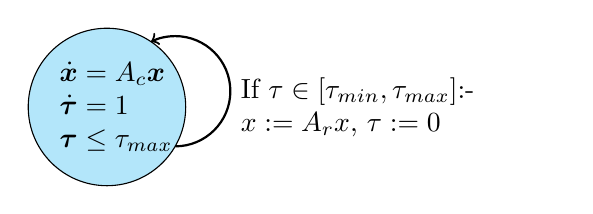
\begin{tikzpicture}
\draw[fill=cyan!30] (0,0) circle (1cm);
\node[text width = 2cm] at (0.4,0) {$\dot{\bm{x}} = A_c\bm{x}$\\$\dot{\bm{\tau}}=1$\\$\bm{\tau}\leq\tau_{max}$};
\draw[thick,->,rotate around={-90:(0,0)}] (0.5,0.867) arc (0:206:0.7);
\node[text width=4cm] at (3.7,0) {If $\tau\in\lt[\tau_{min},\tau_{max}\rt]$:-\\$x:=A_rx$,~$\tau:=0$};
%
\end{tikzpicture}
\hspace{2em}
%
\end{minipage}
%
\emph{}
%
\begin{minipage}{0.48\textwidth}
%
\begin{block}{Global exponential stability (GES)}
Exists \eqnemph{$\lambda\in[0,1)$ and $c>0$} such that \eqnemph{$\forall ~\tbf{x}_0,
\in\mb{R}^n,~k\in\mb{Z}_+$}
\center{\eqnemph{$||\tbf{x}_k||\leq c\lambda^k||\tbf{x}_0||$}}
%
\end{block}
%
\end{minipage}
%
\begin{minipage}{0.48\textwidth}
%
\begin{center}
\vspace{-2em}
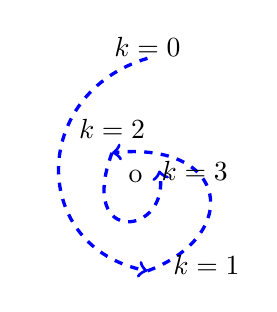
\begin{tikzpicture}[scale=1.5]
\draw[very thick,blue,->,dashed] (0,1)..controls (-1,0.7) and (-1,-0.6)..(0,-0.8);
\draw[very thick,blue,->,dashed] (0,-0.8)..controls (0.8,-0.5) and (0.7,0.3)..(-0.3,0.2);
\draw[very thick,blue,->,dashed] (-0.3,0.2)..controls (-0.6,-0.6) and (0.2,-0.5)..(0.1,0.05);
\node at (-0.1,0) {o};
\node at (0,1.1) {$k=0$};
\node at (0.5,-0.75) {$k=1$};
\node at (-0.3,0.4) {$k=2$};
\node at (0.4,0.05) {$k=3$};
\end{tikzpicture}
\end{center}
%
\end{minipage}
%
\end{frame}

%==================================================================================================================================

\begin{frame}{Set Contraction and Stability Verification}
% \plemph{Reachability operator}
%
%\begin{center}
\eqnemph{$H_\tau=e^{A_c\tau}A_r$.} {Contractive $C$-set}~\cite{2014-fiacchini-set}:
%\end{center}
%
%\emph{}
%

\begin{minipage}{0.48\textwidth}
%
\begin{exampleblock}{}
\plemph{Compact} and \plemph{convex} set $\Psi$:
%
\begin{enumerate}
\item \plemph{Origin} is \plemph{interior} point.
\item \plemph{Contraction}: $\exists~\lambda\in [0,1)$: $\forall \tau\in\lt[\tau_{min},\tau_{max}\rt]$\\
%
\begin{center}
\eqnemph{$H_\tau\Psi\subseteq\lambda\Psi$}.
\end{center}
%
\end{enumerate}
%
\end{exampleblock}
%
\end{minipage}
%
\begin{minipage}{0.48\textwidth}
%
\begin{center}
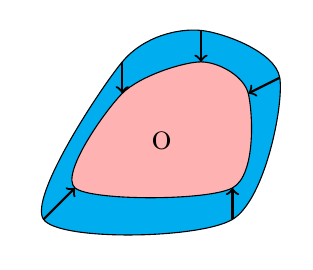
\begin{tikzpicture}[scale=2]
\draw[fill=cyan] plot[smooth cycle] coordinates {(0,0) (0.5,1)
(1,1.2) (1.5,0.9) (1.2,0) };
\draw[fill=red!30] plot[smooth cycle] coordinates {(0.2,0.2) (0.5,0.8)
(1,1) (1.3,0.8) (1.2,0.2) };
\draw[->,thick] (0,0)--(0.2,0.2);
\draw[->,thick] (0.5,1)--(0.5,0.8);
\draw[->,thick] (1,1.2)--(1,1);
\draw[->,thick] (1.5,0.9) -- (1.3,0.8);
\draw[->,thick] (1.2,0)--(1.2,0.2);
\node at (0.75,0.5) {{\Large o}};
\end{tikzpicture}
\end{center}
%
\end{minipage}
%
%\emph{}
%
\begin{alertblock}{}
Existence of \plemph{contractive $C$-set} \eqnemph{$\equivalent$} \plemph{GES}.
\end{alertblock}
%
\begin{itemize}
\item Find \posemph{contractive $C$-set} to \posemph{verify GES}.
\end{itemize}
%
\end{frame}

%==================================================================================================================================

\begin{frame}{Stability Verification Using Complex Zonotope}
%
\begin{center}
{2 stages}:
\begin{enumerate}
\item \plemph{Synthesize} a \plemph{candidate complex zonotope}.
\item \plemph{Verify contraction} of candidate complex zonotope.
\end{enumerate}
\end{center}
%
\end{frame}

%==================================================================================================================================

\begin{frame}{Synthesizing Candidate Complex Zonotope}
%
%\begin{itemize}
%\item \underline{Criterion}: The candidate complex zonotopes should \plemph{contract} with respect to a \plemph{few uniformly sampled reference operators} and be a \plemph{$C$-set}.
%
\begin{enumerate}
\item Collect \plemph{eigenvectors} of \plemph{$K$-uniformly sampled reachability operators} as \plemph{template}.
%
\begin{center}
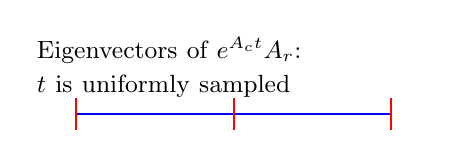
\begin{tikzpicture}[scale=4]
\draw[thick,blue] (0,0)--(1,0);
\draw[thick,red] (0,-0.05)--(0,0.05);
\draw[thick,red] (0.5,-0.05)--(0.5,0.05);
\draw[thick,red] (1,-0.05)--(1,0.05);
\node[text width = 5cm] at (0.5,0.15) {{\small Eigenvectors of ${e^{A_ct}A_r}$:\\ $t$ is uniformly sampled}};
%\draw[dashed,thick,<->] (0.3,-0.1)--(0.7,-0.1);
\end{tikzpicture}
\end{center}
%
%\begin{block}{}
%% \eqnemph{
%% \begin{center}
%%   $\eigenvectors_k$: Eigenvectors of $\omega^k_i=e^{A_c\lt(\lsb+i\frac{(\usb-\lsb)}{k}\rt)}A_r~~\forall i\in\set{0,...,k-1}$.
%% \end{center}
%% }
%\end{block}
%
\item \plemph{Synthesize scaling factors} such that we get
%
\begin{enumerate}
%
\item  \plemph{$\lambda$-contractive} complex zonotope 
\item contains \plemph{unit box} containing origin (\plemph{$C$-set})
%\eqnemph{
%% \begin{center}
%% $\tcztope{\identity{n}{n}}{0}{\repmat{1}{n}{1}}\order\tcztope{\eigenvectors_k}{0}{\sfact}$ \plemph{($C$-set)}\\
%% $\forall t\in\Lambda_k,~ \tcztope{H_t\eigenvectors_k}{0}{\sfact}\order\tcztope{\eigenvectors}{0}{\lambda\sfact}$ \plemph{(contraction)}.
%% \end{center}
%}
%
\end{enumerate}
%
\end{enumerate}
%
%\end{itemize}
%
\end{frame}

%==================================================================================================================================

\begin{frame}{Verifying Contraction w.r.t All Reachability Operators}
%
\begin{enumerate}
\item Derive \plemph{contraction bound} in a small \plemph{neighborhood} of a reachability operator \plemph{using known operations} on complex zonotopes.
%
\begin{itemize}
\item Requires \posemph{convex optimization}.
\end{itemize}
%
\item \plemph{Dynamically} divide \plemph{sampling intervals} into {small sub-intervals} \plemph{while verifying contraction bound $<1$}.
\end{enumerate}
%
\begin{center}
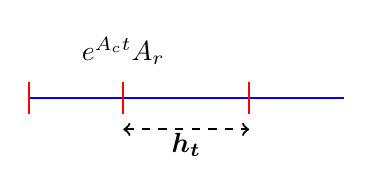
\begin{tikzpicture}[scale=4]
\draw[thick,blue] (0,0)--(1,0);
\draw[thick,red] (0,-0.05)--(0,0.05);
\draw[thick,red] (0.3,-0.05)--(0.3,0.05);
\draw[thick,red] (0.7,-0.05)--(0.7,0.05);
\node at (0.3,0.15) {${e^{A_ct}A_r}$};
\draw[dashed,thick,<->] (0.3,-0.1)--(0.7,-0.1);
\node at (0.5,-0.15) {$\bm{h_t}$};
\end{tikzpicture}
%
\end{center}
\eqnemph{$h_t=$  Maximum interval at $t$} for which \eqnemph{contraction bound} is \eqnemph{less than 1}.
%
\end{frame}

%==================================================================================================================================

\begin{frame}{Benchmark: Networked Control System}
Benchmark from
%Bj\"{o}rn et. al.
~\cite{wittenmark2002computer}

\begin{itemize}
\item Lower bound on the transmission period: $0.08$
\end{itemize}
%
\begin{alertblock}{}
Find \plemph{upper bound $t_{max}$ on transmission period}  such that
system is \plemph{GES}
\end{alertblock}
%
\begin{table}
%\resizebox{\textwidth}{!}{
\begin{tabular}{|l|c|r|}
  \hline
  Reference & $t_{min}$ & $t_{max}$ \\
\hline
  %& &\\
Value recommended in~\cite{wittenmark2002computer} & 0.08 & 0.22\\
  \hline
  %& &\\
  NCS toolbox~\cite{BauLoo_NECSYS12a} & 0.08 & 0.4 \\
\hline
  %& &\\
  Template complex zonotope & 0.08 & 0.58 \\
  \hline
\end{tabular}
%\caption{Experimental results: Example 1}
%}
\end{table}
%
\end{frame}

%==================================================================================================================================

\begin{frame}{Plan}
%
\begin{enumerate}
\item  \plemph{Dynamics} of \plemph{embedded/cyber-physical} systems %\vspace{-1em}
%
%% \begin{itemize}
%% \item \plemph{hybrid system} models, \plemph{trajectory set computation}
%% \end{itemize}
%% %
\emph{}
%
\item \plemph{Usual zonotope} $\rightarrow$ \plemph{Complex zonotope}
%
%% \begin{itemize}
%% \item Capture \plemph{contraction} along \plemph{complex eigenvectors}
%% \end{itemize}
%
%\emph{}
%
\item \plemph{Complex zonotope} $\rightarrow$ \plemph{Template complex zonotope}
%% \begin{itemize}
%% \item Motivation: \plemph{better approximation} of reachable sets
%% \item Basic \posemph{operations}: linear transformation, Minkowski sum, support function
%% \item \plemph{Checking inclusion} : \posemph{convex program}
%% \end{itemize}
%% %
%% \emph{}
%
\item \plemph{Template Complex Zonotope} $\rightarrow$ \plemph{Augmented complex zonotope}
%% %
%% \begin{itemize}
%% \item \posemph{Intersection} with \posemph{linear constraints}
%% \end{itemize}
%% %
%% \emph{}
%% %
\begin{alertblock}{}
\item \plemph{Applications}:
%
\begin{itemize}
\item {\posemph{Stability verification} of \plemph{networked control} systems}
%\item \posemph{Computing positive invariants} of discrete time affine hybrid systems
\item \fbox{\posemph{Verification of linear invariance property} of   affine hybrid systems}
\end{itemize}
\end{alertblock}
%
\end{enumerate}
%
\end{frame}

%==================================================================================================================================

%\subsection{Invariance Verification for Affine Hybrid System}

\begin{frame}{Checking Positive Invariance for Affine Hybrid System}
%% %
%% \begin{minipage}{0.45\textwidth}
%% \plemph{Continuous transition}:

%% %
%% \begin{tikzpicture}
%% \draw[fill=red] (0,0) circle (0.7);
%% \node at (0,0) {{\Large $q$}};
%% \node[text width = 4cm] at (0,1) {Stay: $x\in\ptope{\qtemp}{\lb_q}{\ub_q}$};
%% \node[text width = 5cm] at (0,-1) {{ \hspace{3em}$A_q x\oplus\acztope{\ptemp_q^{\operatorname*{inp}}}{\cen_q^{\operatorname*{inp}}}{\sfact_q^{\operatorname*{inp}}}{\stemp_q^{\operatorname*{inp}}}{\lb_q^{\operatorname*{inp}}}{\ub_q^{\operatorname*{inp}}}$}};
%% \end{tikzpicture}
%% %
%% %% \begin{align*}
%% %% & \exists l^\pr_q,u^\pr_q:\\
%% %% & \mathcal{G}\lt(\begin{array}{l}
%% %% \mymatrix{A\ptemp_q & \ptemp_q^{\operatorname*{inp}}},{A\cen_q+\cen_q^{\operatorname*{inp}}},{\mymatrix{\sfact\\\sfact_q^{\operatorname*{inp}}}}\\
%% %% {\mymatrix{\stemp_q & \stemp_q^{\operatorname*{inp}}}},{\mymatrix{\lb\\\lb_q^{\operatorname*{inp}}}},{\mymatrix{\ub\\\ub_q^{\operatorname*{inp}}}}
%% %% \end{array}
%% %% \rt)
%% %% \end{align*}
%% \end{minipage}
%% %
%% \hspace{0.5em}\vline\hspace{0.5em}
%% %
%% \begin{minipage}{0.45\textwidth}
%% \plemph{Discrete transition}:

%% \begin{tikzpicture}
%% \draw[fill=red] (-1,0) circle (0.5);
%% \draw[fill=red] (1,0) circle (0.5);
%% \draw[thick,->] (-0.5,0)--(0.5,0);
%% \node at (-1,0) {{\Large ${\sigma_1}$}};
%% \node at(1,0) {{\Large ${\sigma_2}$}};
%% \node[text width = 6cm] at (1,1) {Respective Staying conditions;\\ Guard: $x\in\ptope{\qtemp}{\lb_\sigma}{\ub_\sigma}$;};
%% \node[text width = 5cm] at (1,-1) {{ \hspace{3em}$A_\sigma x\oplus\acztope{\ptemp_\sigma^{\operatorname*{inp}}}{\cen_\sigma^{\operatorname*{inp}}}{\sfact_\sigma^{\operatorname*{inp}}}{\stemp_\sigma^{\operatorname*{inp}}}{\lb_\sigma^{\operatorname*{inp}}}{\ub_\sigma^{\operatorname*{inp}}}$}};
%% \end{tikzpicture}
%% %
%% \end{minipage}
%
Involves:
\begin{itemize}
\item \plemph{Intersection} with \plemph{guards} and \plemph{staying conditions}
\item \plemph{Affine transition} under {additive disturbance}
\end{itemize}
\pause
%
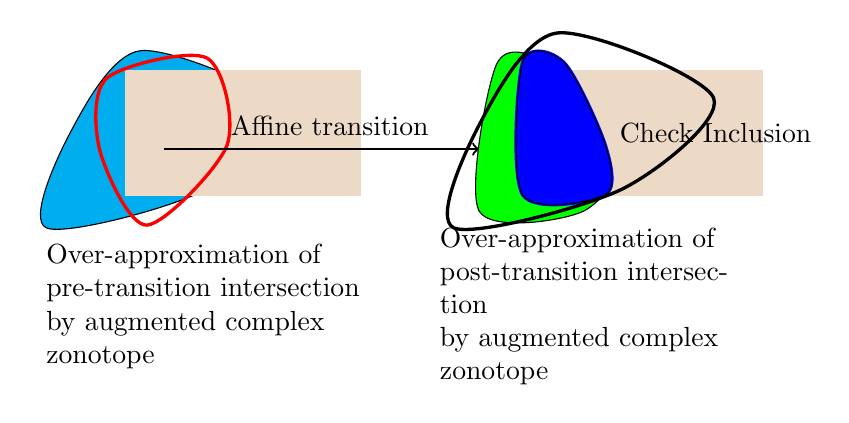
\begin{tikzpicture}
\draw[fill=cyan,scale=1.5] plot[smooth cycle] coordinates{(0,0) (0.2,0.8) (0.8, 1.5) (2, 1) (1.3, 0.3)};
\pause
\fill[fill=brown!30,scale=2] (0.5,0.2) rectangle (2,1);
\draw[very thick, red, rotate around = {45:(2,2)},xshift=0.1cm, yshift=1cm,scale=1.2] plot[smooth cycle] coordinates{(0,0.1) (0.2,1) (0.8, 1.5) (1.7,0.9) (1.2, 0.1)};
\node[text width=4cm] at (2,-1) {Over-approximation of pre-transition intersection\\by augmented complex zonotope};
\pause
\draw[->,yshift=1cm,xshift=0.5cm,thick] (1,0)--(5,0);
\node at (3.6,1.3) {Affine transition};
\draw[fill = green,rotate around = {0:(2,2)},xshift=5.5cm, yshift=0.1cm,scale=1.1] plot[smooth cycle] coordinates{(0,0.1) (0.2,1.8) (0.8, 1.8) (1.7,0.9) (1.2, 0.1)};
\pause
\fill[fill=brown!30,scale=2,xshift=2.55cm,yshift=0.1] (0.5,0.2) rectangle (2,1);
\draw[very thick, color=blue, xshift=5cm, scale=2.1] plot [smooth cycle] coordinates{(0.5,0.2) (0.5,1)  (0.75,1) (1,0.5) (1,0.2)};
\node[text width=4cm] at (7,-1) {Over-approximation of post-transition intersection\\by augmented complex zonotope};
\pause
\draw[fill=blue, xshift=5cm, scale=2.1] plot [smooth cycle] coordinates{(0.5,0.2) (0.5,1)  (0.75,1) (1,0.5) (1,0.2)};
\draw[very thick, black, scale=1.5,xshift=3.45cm,yshift=0cm,scale=1.1] plot[smooth cycle] coordinates{(0,0) (0.2,0.8) (0.8, 1.5) (2, 1) (1.3, 0.3)};
\node at (8.5,1.2) {Check Inclusion};
\end{tikzpicture}
%
\end{frame}

%==================================================================================================================================

\begin{frame}{Verifying Linear Invariance by Convex Optimization}
%
\begin{minipage}{0.48\textwidth}
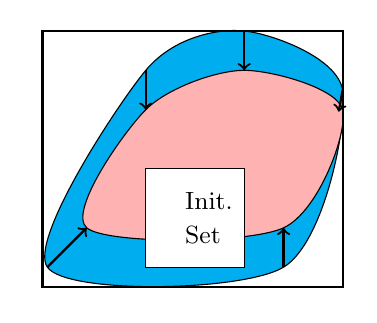
\begin{tikzpicture}[scale=2.5]
\draw[fill=cyan] plot[smooth cycle] coordinates {(0,0) (0.5,1)
(1,1.2) (1.5,0.9) (1.2,0) };
\draw[fill=red!30] plot[smooth cycle] coordinates {(0.2,0.2) (0.5,0.8)
(1,1) (1.5,0.8) (1.2,0.2) };
\draw[->,thick] (0,0)--(0.2,0.2);
\draw[->,thick] (0.5,1)--(0.5,0.8);
\draw[->,thick] (1,1.2)--(1,1);
\draw[->,thick] (1.5,0.9) -- (1.48,0.79);
\draw[->,thick] (1.2,0)--(1.2,0.2);
\draw[fill=white] (0.5,0) rectangle (1,0.5);
\node[text width = 0.25cm] at (0.75, 0.25) {\small Init.\\ Set };
\draw[thick] (-0.025 ,-0.1) rectangle (1.5,1.2);
\end{tikzpicture}
\end{minipage}
%
\begin{minipage}{0.48\textwidth}
\plemph{Linear Invariance}: All \plemph{reachable states} satisfy \plemph{linear constraints}\\[1em]
Verification using\\ \fbox{\posemph{Single step of convex optimization}}
\end{minipage}
\emph{}
%
\begin{enumerate}
\item Fix templates of complex zonotope.
\begin{itemize}
\item Secondary template is \plemph{pseudo-inverse} of primary template.
\item Choice of \plemph{primary template} according to \plemph{dynamics}.
\end{itemize}
\emph{}
\item Write \plemph{convex constraints}  for \plemph{operations} \\
1) \plemph{positive invariance} 2) \plemph{inclusion} of \plemph{initial set} 3) \plemph{inclusion} inside \plemph{linear constraints}
\end{enumerate}
%
\end{frame}

%==================================================================================================================================

\begin{frame}{Choice of Primary Template}
%% \begin{itemize}
%% \item \textcol{Secondary template} is fixed as \textcol{Pseudo-Inverse} of \textcol{Sub-Parallelotopic template} of \plemph{guards} and \plemph{staying conditions}.\emph{}
%% \end{itemize}
\begin{block}{}
\begin{enumerate}
\item \plemph{Eigenvectors} of the transformation matrices and their products, \plemph{templates} of \plemph{input sets}
\item  \plemph{Orthogonal projections}  on the null space of
   the \plemph{parallelotope template} of \plemph{guards} and \plemph{staying conditions}  
\item  \plemph{Additional} vectors
\end{enumerate}
\end{block}

\end{frame}


%\section{Benchmarks}

\begin{frame}{Benchmark 1: NXT-Lego Robot Model}
\eqncol{Benchmark example} published in \eqncol{ARCH 2014~\cite{heinz2014benchmark}} %\textcol{(Heinz, Oehlerking and Woehrle.)}

\begin{minipage}{0.3\textwidth}
\begin{figure}
\centering
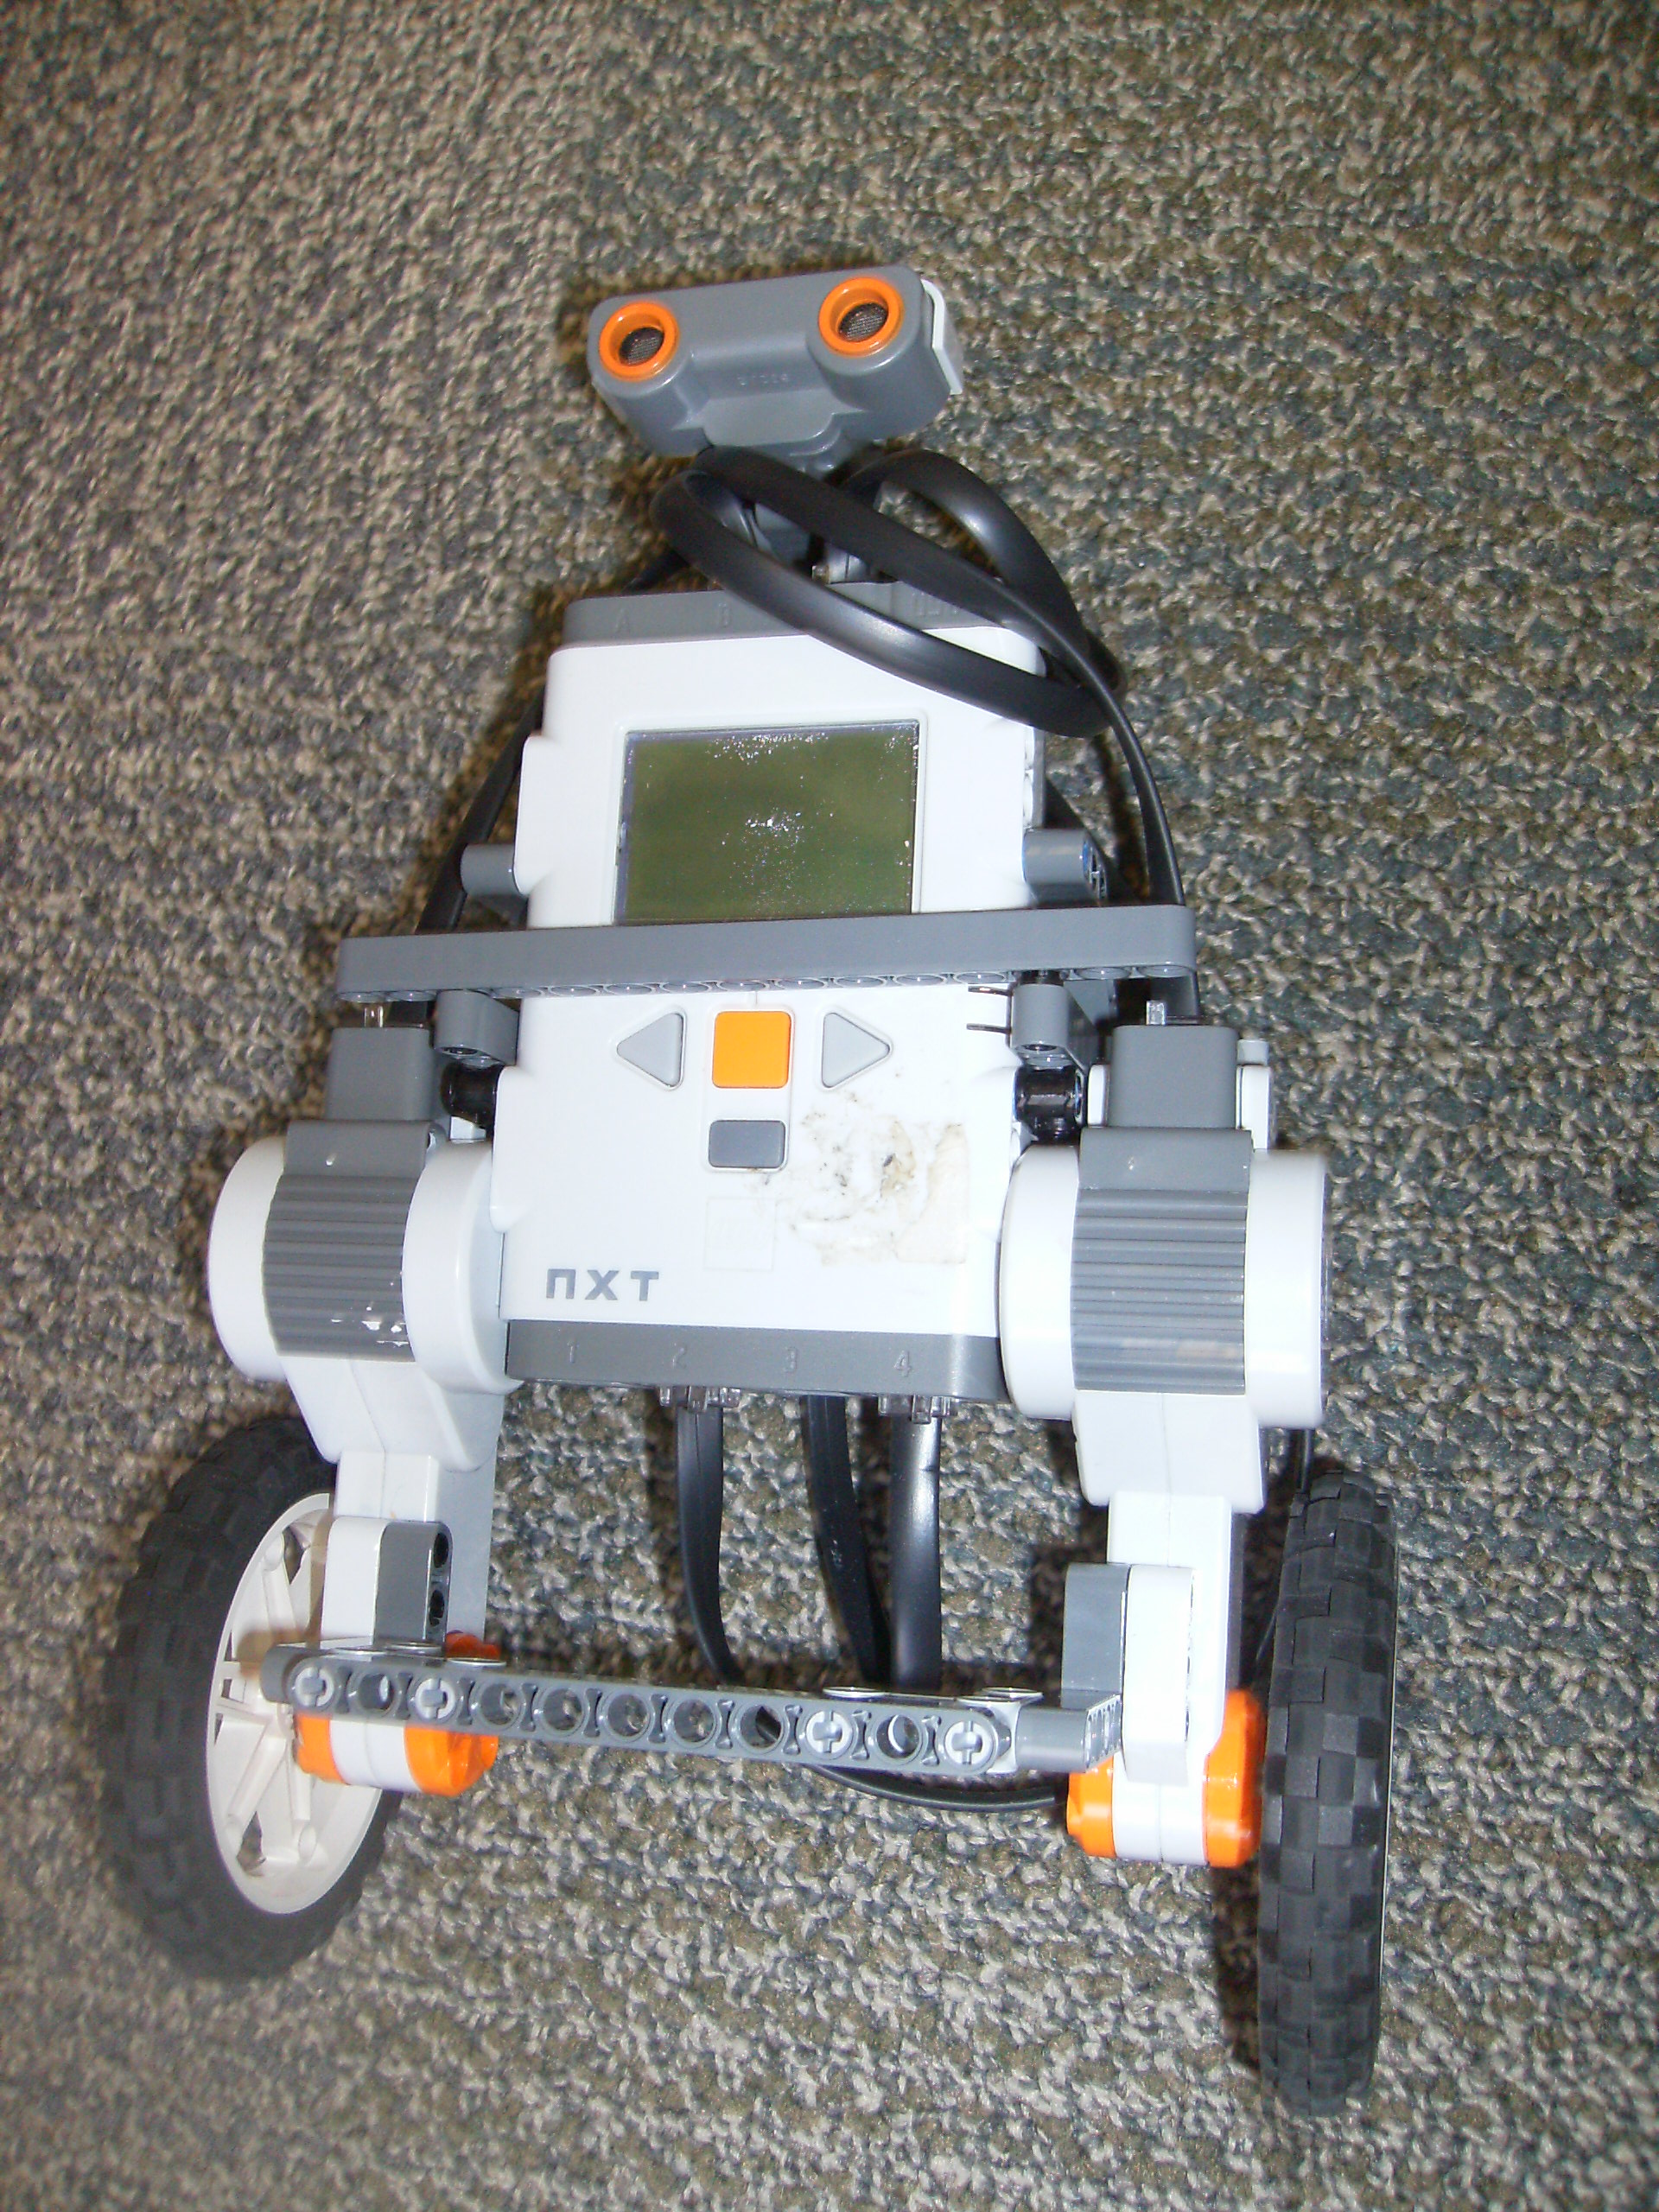
\includegraphics[scale=0.09]{fig/NXT-lego.JPG}
\end{figure}
\end{minipage}
\begin{minipage}{0.6\textwidth}
{\footnotesize Lego NXT self-balancing robot by\\ Medelen8/CC-BY-SA-3.0}
\begin{itemize}
\item \textcol{Sampled data Networked Control System}:
\item Controller input has \textcol{saturation} on {\color{violet} 2 controller inputs}: \textcol{hybrid behavior}.
\end{itemize}
\end{minipage}

%% \begin{block}{}
%% $
%% \lt[\begin{array}{cc}\trj{x}{t+1} &
%%     \trj{y}{t+1}\end{array}\rt]^T=F_1\trj{x}{t}+F_2sat\lt(\trj{y}{t}\rt)+F_3\trj{u}{t}$\\
%% \textcol{Saturated}: $sat\lt(y_i\rt) = max\lt(-\delta
%% d_p,min\lt(y_i,\delta d_p\rt)\rt),~\forall i\in\{1,2\}$, where $\delta=100$
%% and $d_p=0.0807$. \textcol{Unsaturated}: $sat\lt(y_i\rt) = y_i$
%% \end{block}
\end{frame}


\begin{frame}{NXT-Lego Robot Model: Verification Problem}
\begin{alertblock}{}
Verify bounds on \textcol{body pitch angle}
\end{alertblock}
%
\eqncol{After transformation to decouple unbounded directions, we
obtained}\\
%
\begin{block}{Complexity}
\begin{itemize}
\item \eqncol{Saturated}: \textcol{9 dimensional, 1 location, 9 edges.}
\item \eqncol{Unsaturated}: \textcol{9 dimensional linear system.}
\end{itemize}
\end{block}
%
\end{frame}

%% \begin{frame}{Experimental settings}
%% %
%% \begin{itemize}
%% \item \eqncol{Primary template:}  (Complex) \textcol{Eigenvectors} of linear maps and their products,
%%  \textcol{Orthonormal
%% vectors} to guarding hyperplane normals.  For
%% the linear system, it consists of the eigenvectors of the linear map,
%% the \textcol{uncertain input set template} and its multiplication by the linear matrix
%% (related to affine map) and square of the linear matrix. 
%% \item \eqncol{SpaceEx settings:}  \textcol{Octagon template} and a
%% template with \textcol{$400$ uniformly sampled support vectors}.
%% \end{itemize}
%% %
%% \end{frame}

%==================================================================================================================================

\begin{frame}{NXT-Lego Robot Model: Results}
\center{{\eqncol{\small{\footnotesize UB: $>$1000, ~~NT: Not terminating in more than 180s, \newline
  n/a: Not applicable/not available, ~~ACZ: Augmented complex
  zonotope.}}}}
{\color{black}
\begin{minipage}{0.48\textwidth}
\begin{table}
\centering
\resizebox{0.5\textheight}{0.35\textwidth}{
\begin{tabular}{|l|c|c|c|}
\hline
\multicolumn{2}{|c|}{\multirow{2}{*}{Method}} &
\multirow{2}{*}{$\lt|\psi\rt|\leq$} & Comp.\\
\multicolumn{2}{|c|}{} & & time (s)\\
\hline
\multirow{4}{*}{SpaceEx} & octagon & \multirow{2}{*}{UB} & \multirow{2}{*}{NT}\\
& template & & \\
\cline{2-4}
& 400 support & \multirow{2}{*}{UB} & \multirow{2}{*}{NT}\\
& vectors & &\\
\hline
\multicolumn{2}{|c|}{\multirow{2}{*}{Suggested in~\cite{heinz2014benchmark}}} &
\multirow{2}{*}{$1.39$} & \multirow{2}{*}{n/a}\\
\multicolumn{2}{|c|}{} & &\\
\hline
\multicolumn{2}{|c|}{\multirow{2}{*}{ACZ invariant}} & \multirow{2}{*}{$1.29$} &
\multirow{2}{*}{$4$}\\
\multicolumn{2}{|c|}{} & & \\
\hline
\end{tabular}
}
\caption*{{\footnotesize Unsaturated robot model: results}}
\end{table}
\end{minipage}
\begin{minipage}{0.48\textwidth}
\begin{table}
\centering
\resizebox{0.5\textheight}{0.35\textwidth}{
\begin{tabular}{|l|c|c|c|}
\hline
\multicolumn{2}{|c|}{\multirow{2}{*}{Method}} &
\multirow{2}{*}{$\lt|\psi\rt|\leq$} & Comp.\\
\multicolumn{2}{|c|}{} & & time (s)\\
\hline
\multirow{4}{*}{SpaceEx} & octagon & \multirow{2}{*}{UB} &
\multirow{2}{*}{NT}\\
& template & & \\
\cline{2-4}
& 400 support & \multirow{2}{*}{UB} & \multirow{2}{*}{NT}\\
& vectors & & \\
\hline
\multicolumn{2}{|c|}{\multirow{2}{*}{Suggested in~\cite{heinz2014benchmark}}} &
$1.571-\epsilon:$ & \multirow{2}{*}{n/a}\\
\multicolumn{2}{|c|}{} & $\epsilon>0$ &\\
\hline
\multicolumn{2}{|c|}{\multirow{2}{*}{ACZ invariant}} & \multirow{2}{*}{$1.13$} &
\multirow{2}{*}{45}\\
\multicolumn{2}{|c|}{} & &\\
\hline
\end{tabular}
}
\caption*{{\footnotesize Saturated robot model: results}}
\end{table}
\end{minipage}
}
\vspace{-2em}
{\small
\begin{alertblock}{Remarks}
\begin{itemize}
\item Model has \textcol{complex eigenstructure}, some eigenvalues have \textcol{magnitude close to 1}.
\item \textcol{Complex Zonotope uses complex eigenstructure}: better \plemph{accuracy}.
\end{itemize}
\end{alertblock}
}
\end{frame}

%==================================================================================================================================

\begin{frame}{Benchmark 2: Networked Vehicle Platoon}
\begin{figure}
\caption*{\small Benchmark {\color{blue}  2014 ARCH Workshop}: \eqncol{~\cite{makhlouf2014networked}}}
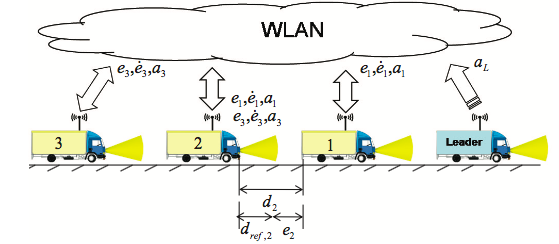
\includegraphics[scale=0.4]{fig/VehiclePlatoon.png}\\
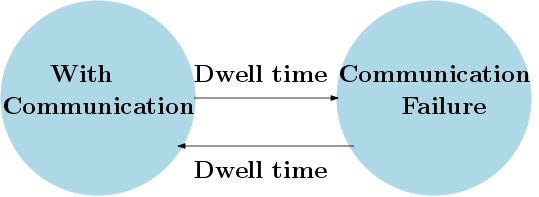
\includegraphics[scale=0.4]{fig/networked-platoon-model.png}
\end{figure}
\end{frame}

%==================================================================================================================================

\begin{frame}{Networked Platoon Verification Problem}
\begin{alertblock}{}
%\begin{itemize}
%\item
Verify \textcol{reference distances} between vehicles such that they \plemph{ do not collide}.
%\end{itemize}
\end{alertblock}
%
\begin{exampleblock}{Two cases}
\begin{enumerate}
\item \textcol{Slow switching}: \eqncol{Minimum dwell time 20 s}. {\color{violet} 9 dimensional, 2 locations, 4 edges}.
\item \textcol{Fast switching}: \eqncol{Integer dwell times}. {\color{violet} 9 dimensional, 2 locations, 2 edges}.
\end{enumerate}
\end{exampleblock}
\end{frame}

\begin{frame}{Networked Platoon: Results}
\begin{table}
\resizebox{1.1\textwidth}{!}{\hspace{-3em}
\begin{tabular}{|l|c|c|c|c|c|c|c|c|c|}
\hline
\multicolumn{2}{|c|}{\multirow{4}{*}{Method}} & \multicolumn{4}{|c|}{\multirow{2}{*}{Slow switching}} & \multicolumn{4}{|c|}{\multirow{2}{*}{Fast switching}}\\
\multicolumn{2}{|c|}{} & \multicolumn{4}{|c|}{} & \multicolumn{4}{|c|}{} \\
\cline{3-10}
\multicolumn{2}{|c|}{} & \multirow{2}{*}{$-e_1\leq$} & \multirow{2}{*}{$-e_2\leq$} & \multirow{2}{*}{$-e_3\leq$} & Comp. & \multirow{2}{*}{$-e_1\leq$} & \multirow{2}{*}{$-e_2\leq$} & \multirow{2}{*}{$-e_3\leq$} & Comp.\\
\multicolumn{2}{|c|}{} & & & & time (s) & & & & time (s)\\
\hline
\multirow{4}{*}{SpaceEx} & octagon & \multirow{2}{*}{28} &
\multirow{2}{*}{27} & \multirow{2}{*}{10} &
\multirow{2}{*}{NT} & \multirow{2}{*}{UB} &
\multirow{2}{*}{UB} & \multirow{2}{*}{UB} &
\multirow{2}{*}{NT}\\
& template & & & & & & & &\\
\cline{2-10}
& 100 support & \multirow{2}{*}{28} & \multirow{2}{*}{25} &
\multirow{2}{*}{13} & \multirow{2}{*}{1.3} & \multirow{2}{*}{UB} & \multirow{2}{*}{UB} &
\multirow{2}{*}{UB} & \multirow{2}{*}{NT}\\
& vectors & & & & & & & &\\
\hline
\multicolumn{2}{|c|}{\multirow{2}{*}{Real zonotope~\cite{makhlouf2014networked}}} &
\multirow{2}{*}{25} & \multirow{2}{*}{25} & \multirow{2}{*}{10}
 & \multirow{2}{*}{n/a} & \multirow{2}{*}{n/a} & \multirow{2}{*}{n/a} & \multirow{2}{*}{n/a}
 & \multirow{2}{*}{n/a}\\
\multicolumn{2}{|c|}{} & & & & & & & &\\
\hline
\multicolumn{2}{|c|}{\multirow{2}{*}{ACZ invariant}} &
\multirow{2}{*}{28} & \multirow{2}{*}{26} &
\multirow{2}{*}{12} & \multirow{2}{*}{12} &
\multirow{2}{*}{46} & \multirow{2}{*}{54} &
\multirow{2}{*}{57} & \multirow{2}{*}{12.6}\\
\multicolumn{2}{|c|}{} & & & & & & & &\\
\hline
\end{tabular}
}
%% \caption*{{\footnotesize UB: $>$1000, ~~NT: Not terminating in more than 180s, \newline
%%   n/a: Not applicable/not available, ~~ACZ: Augmented complex
%%   zonotope.
%% }}
{\small
\begin{alertblock}{Remarks}
\begin{itemize}
\item {\bf Fast switching model} is \textcol{less stable} than  {\bf slow switching model} 
\item Since {\bf complex zonotope} used \textcol{eigenstructure}: better \plemph{accuracy} on \plemph{less stable} model
\end{itemize}
\end{alertblock}
}
\end{table}
\end{frame}

%==================================================================================================================================

%% \begin{frame}{Perturbed double integrator}
%% \begin{itemize}
%% \item Example from \textcol{CDC 2004}~\cite{rakovic2004computation}.
%% \item \textcol{Piecewise affine with 2 dimensional additive disturbance input}, \eqncol{Four different Affine
%% dynamics} in \eqncol{Four different polytopic regions} of space.
%% \item Model complexity: \textcol{2 dimensions, 4 locations and 12 edges.}
%% \end{itemize}
%% \begin{alertblock}{Challenge}
%% \begin{enumerate}
%% \item Verify \textcol{smallest (possible) bounds} on the \textcol{two state space co-ordinates}.
%% \item Compute a \textcol{large set} of \textcol{safe initial conditions}.
%% \end{enumerate}
%% \end{alertblock}
%% \emph{}
%% \begin{exampleblock}{Experimental settings}
%% \begin{itemize}
%% \item  {\bf Primary template}: \textcol{Complex eigenvectors} of all linear matrices of the \textcol{affine maps and
%% their binary products}. 
%% \item  {\bf SpaceEx tool}: \eqncol{Two
%% different templates}: \textcol{Octagon} template and a template with \textcol{100
%% uniformly sampled support vectors}.
%% \end{itemize}
%% \end{exampleblock}
%% \end{frame}

%% \begin{frame}{Experimental results: PDI}
%% \begin{table}
%% \begin{minipage}{\textwidth}
%% \center
%% \caption*{Small invariant computation}
%% {\small
%% \begin{tabular}{|l|c|c|c|c|}
%% \hline
%% \multicolumn{2}{|c|}{\multirow{2}{*}{Method}} &
%% \multirow{2}{*}{$\lt|x_1\rt|\leq$} & \multirow{2}{*}{$\lt|x_2\rt|\leq$} & Comp.\\
%% \multicolumn{2}{|c|}{} & & & time (s) \\
%% \hline
%% \multirow{4}{*}{SpaceEx} & octagon & \multirow{2}{*}{0.38} &
%% \multirow{2}{*}{0.43} & \multirow{2}{*}{1.7}\\
%% & template & & &\\
%% \cline{2-5}
%% & 100 support & \multirow{2}{*}{0.38} & \multirow{2}{*}{0.43} & \multirow{2}{*}{23.6}\\
%% & vectors & & &\\
%% \hline
%% \multicolumn{2}{|c|}{\multirow{2}{*}{ACZ invariant}} &
%% \multirow{2}{*}{0.36} & \multirow{2}{*}{0.43} & 
%% \multirow{2}{*}{5.1}\\
%% \multicolumn{2}{|c|}{} & & &\\
%% \hline
%% \end{tabular}
%% }
%% \end{minipage}
%% \hspace{4em}
%% \begin{minipage}{\textwidth}
%% \center
%% {\small
%% \caption*{Large invariant computation}
%% \begin{tabular}{|c|c|}
%% \hline
%% \multirow{2}{*}{Method} & Comp.\\
%% & time (s)\\
%% \hline
%% \multirow{2}{*}{MPT tool~\cite{rakovic2004computation}} & \multirow{2}{*}{107}\\
%% & \\
%% \hline
%% \multirow{2}{*}{ACZ} & \multirow{2}{*}{12}\\
%% & \\
%% \hline
%% \end{tabular}
%% }
%% \end{minipage}
%% \end{table}
%% \end{frame}

%==================================================================================================================================



\begin{frame}{Contributions}
\begin{enumerate}
\item \posemph{Complex zonotope representations} that
\begin{itemize}
\item capture continuous dynamics contractions 
\item efficient operations for discrete dynamics
\end{itemize}


\item Improve the \plemph{state of the art} of \plemph{verification}
%% \begin{itemize}
%% \item Captures \posemph{contraction} along \posemph{complex eigenvectors}.
%% \item \posemph{Linear transformation} and \plemph{Minkowski sum} are \plemph{efficiently computable}.
%% \end{itemize}
%
%\emph{}
%\item \posemph{Template based representation} for \posemph{finding better approximations}
%\emph{}
%\item \posemph{Intersection with linear constraints} using \posemph{augmented complex zonotope}
%\emph{}
%\item \plemph{Applications}:  Develop \plemph{convex programs} for verifying
%
\begin{enumerate}
%\item \posemph{positive invariance}
\item \posemph{linear invariance}
\item \posemph{stability}
 \end{enumerate}
 %
\item Implementation and successful experimentation on \plemph{benchmarks}
\end{enumerate}
\end{frame}

%==================================================================================================================================

\begin{frame}{Future Work}
\begin{enumerate}
\item Experiment with more \plemph{real world applications}
\item Application to \plemph{abstract interpretation} of \plemph{embedded control programs} by combining with existing tools
\item Extend \plemph{application} of complex zonotopes to \plemph{Non-linear dynamics} and \plemph{Continuous time} hybrid systems
\end{enumerate}
\end{frame}

\begin{frame}{Publications}
\begin{enumerate}
\item Arvind Adimoolam and Thao Dang.
\newblock Augmented complex zonotopes for computing invariants of affine hybrid
  systems.
\newblock In {\em International Conference on Formal Modeling and Analysis of
  Timed Systems}, pages 97--115. Springer, 2017.

\item Arvind Adimoolam, Thao Dang, Alexandre Donz{\'e}, James Kapinski, and Xiaoqing
  Jin.
\newblock Classification and coverage-based falsification for embedded control
  systems.
\newblock In {\em International Conference on Computer Aided Verification},
  pages 483--503. Springer, 2017.


\item %\bibitem{tcz2017}
Arvind Adimoolam and Thao Dang.
\newblock Template complex zonotopes for stability and invariant computation.
\newblock In {\em American Control Conference (ACC), 2017}. IEEE, 2017.


\item %\bibitem{adimoolamACC2016}
Arvind~S Adimoolam and Thao Dang.
\newblock Using complex zonotopes for stability verification.
\newblock In {\em American Control Conference (ACC), 2016}, pages 4269--4274.
  IEEE, 2016.
\end{enumerate}
\end{frame}

%==================================================================================================================================

\begin{frame}{}
\center
{\Huge {\color{blue} Thank you!}}
\end{frame}



\bibliographystyle{apalike}
\bibliography{lib,thesis/reflis}

%% \begin{frame}{Special Case: Interval Zonotope and Sub-parallelotope}
%% %
%% \begin{minipage}{0.45\textwidth}
%% \plemph{Interval Zonotope}: {\small Representation of \plemph{real zonotope} using \plemph{{variable\\ {interval} bounds}}, no explicit center.\\[0.5em]
%% %
%% \eqnemph{${\lb,\ub}\in\reals^k:~\lb\leq \ub$}, ${\stemp\in\mat{k}{n}{\reals}}$.}
%% %
%% {\small
%% \begin{exampleblock}{\center{$\iztope{\stemp}{\lb}{\ub}$}}
%% \eqnemph{$\set{\stemp\zeta:~\zeta\in\reals^k,~\lb\leq\zeta\leq\ub}.$}
%% \end{exampleblock}
%% }
%% %
%% \end{minipage}
%% %
%% \hspace{0.25em}
%% \vline
%% \hspace{0.25em}
%% %
%% \begin{minipage}{0.45\textwidth}
%% \plemph{Sub-parallelotope}: {\small Represents  \\\plemph{possibly unbounded parallelotopes}.\\[0.5em]
%% %
%% \eqnemph{${\plb\in\lt(\reals\bigcup\set{-\infty}\rt)^k}$, ${\pub\in\lt(\reals\bigcup\set{\infty}\rt)^k}$\\[0.5em]
%% %
%% ${\qtemp\in\mat{n}{k}{\reals}:{k\leq n}},~~{\qtemp\transpose{\qtemp}:\text{invertible}}$.
%% }
%% }
%% \vspace{-0.5em}
%% %
%% {\small
%% \begin{exampleblock}{\center{$\ptope{\qtemp}{\plb}{\pub}$}}
%% \eqnemph{$\set{x\in\reals^n:~\plb\leq\qtemp x\leq\pub}$.}
%% \end{exampleblock}
%% }
%% %
%% \end{minipage}
%% %
%% \begin{block}{}
%% \center{\eqnemph{$\lt(\iztope{\pinv{\qtemp}}{\lb}{\ub}\rt)\bigcap\ptope{\qtemp}{\plb}{\pub}
%% =\iztope{\pinv{\qtemp}}{\join{\lb}{\plb}}{\meet{\ub}{\pub}}$}.}
%% \end{block}
%% %
%% \begin{tikzpicture}[scale = 1.5]
%% \node[text width = 3cm] at (-1,0.75) {{\small $\qtemp = \mymatrix{1 & 0\\ -1 & 4}$\\[0.5em]$\lb = \mymatrix{0\\ 0}$ $\ub = \mymatrix{2\\3}$}};
%% \node[text width = 4cm] at (4.5,0.75) {{\small $\plb = \mymatrix{1\\ -\infty}$ $\pub = \mymatrix{\infty\\3}$}};
%% \draw[fill=red!30] (0,0)--(0,1)--(2,1.5)--(2,0.5)--cycle;
%% \fill[cyan] (1,1)--(3,1.5)--(3,-1.5)--(1,-2)--cycle;
%% \draw[dashed, thick, fill = green!30] (1,1)--(2,1.25)--(2,0.5)--(1,0.25)--cycle;
%% \draw[->, thick] (2,1.25)--(2.8,1.45);
%% \draw[->, thick] (1,0.25)--(1,-0.1);
%% \end{tikzpicture}
%% %
%% \end{frame}



\end{document}

